% Created by tikzDevice version 0.12.3.1 on 2022-09-09 15:36:13
% !TEX encoding = UTF-8 Unicode
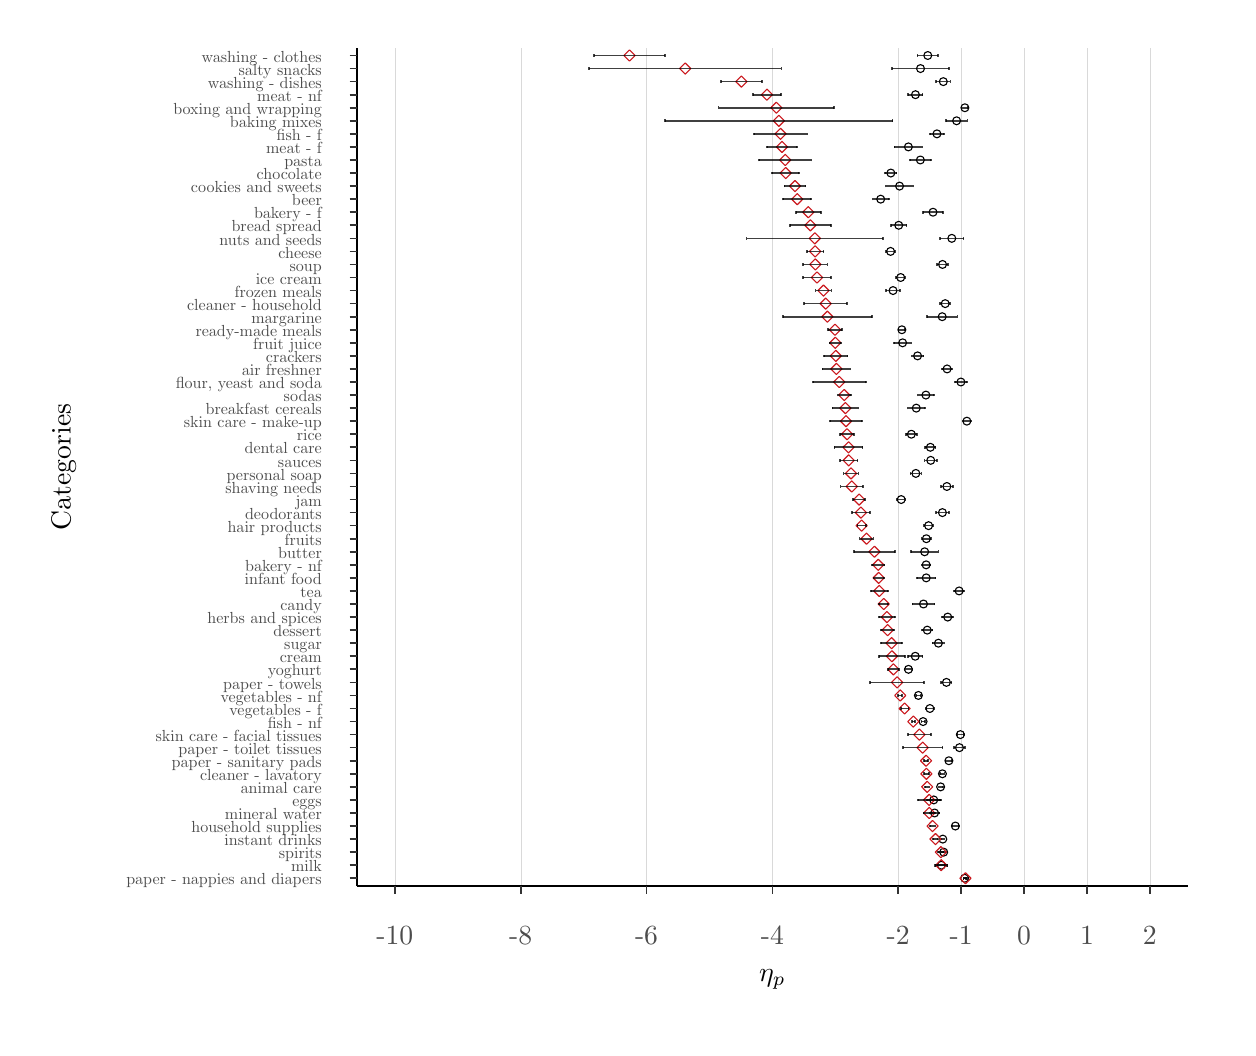
\begin{tikzpicture}[x=1pt,y=1pt]
\definecolor{fillColor}{RGB}{255,255,255}
\path[use as bounding box,fill=fillColor,fill opacity=0.00] (0,0) rectangle (433.62,361.35);
\begin{scope}
\path[clip] (  0.00,  0.00) rectangle (433.62,361.35);
\definecolor{drawColor}{RGB}{255,255,255}
\definecolor{fillColor}{RGB}{255,255,255}

\path[draw=drawColor,line width= 0.6pt,line join=round,line cap=round,fill=fillColor] (  0.00,  0.00) rectangle (433.62,361.35);
\end{scope}
\begin{scope}
\path[clip] (119.04, 51.15) rectangle (419.17,354.12);
\definecolor{drawColor}{RGB}{255,255,255}

\path[draw=drawColor,line width= 0.3pt,line join=round] (155.42, 51.15) --
	(155.42,354.12);

\path[draw=drawColor,line width= 0.3pt,line join=round] (200.89, 51.15) --
	(200.89,354.12);

\path[draw=drawColor,line width= 0.3pt,line join=round] (246.37, 51.15) --
	(246.37,354.12);

\path[draw=drawColor,line width= 0.3pt,line join=round] (291.84, 51.15) --
	(291.84,354.12);

\path[draw=drawColor,line width= 0.3pt,line join=round] (325.95, 51.15) --
	(325.95,354.12);

\path[draw=drawColor,line width= 0.3pt,line join=round] (348.68, 51.15) --
	(348.68,354.12);

\path[draw=drawColor,line width= 0.3pt,line join=round] (371.42, 51.15) --
	(371.42,354.12);

\path[draw=drawColor,line width= 0.3pt,line join=round] (394.16, 51.15) --
	(394.16,354.12);
\definecolor{drawColor}{gray}{0.85}

\path[draw=drawColor,line width= 0.1pt,line join=round] (132.68, 51.15) --
	(132.68,354.12);

\path[draw=drawColor,line width= 0.1pt,line join=round] (178.16, 51.15) --
	(178.16,354.12);

\path[draw=drawColor,line width= 0.1pt,line join=round] (223.63, 51.15) --
	(223.63,354.12);

\path[draw=drawColor,line width= 0.1pt,line join=round] (269.10, 51.15) --
	(269.10,354.12);

\path[draw=drawColor,line width= 0.1pt,line join=round] (314.58, 51.15) --
	(314.58,354.12);

\path[draw=drawColor,line width= 0.1pt,line join=round] (337.31, 51.15) --
	(337.31,354.12);

\path[draw=drawColor,line width= 0.1pt,line join=round] (360.05, 51.15) --
	(360.05,354.12);

\path[draw=drawColor,line width= 0.1pt,line join=round] (382.79, 51.15) --
	(382.79,354.12);

\path[draw=drawColor,line width= 0.1pt,line join=round] (405.52, 51.15) --
	(405.52,354.12);
\definecolor{drawColor}{RGB}{0,0,0}

\path[draw=drawColor,line width= 0.4pt,line join=round,line cap=round] (332.23,238.03) circle (  1.43);

\path[draw=drawColor,line width= 0.4pt,line join=round,line cap=round] (329.89, 87.02) circle (  1.43);

\path[draw=drawColor,line width= 0.4pt,line join=round,line cap=round] (327.14,294.66) circle (  1.43);

\path[draw=drawColor,line width= 0.4pt,line join=round,line cap=round] (324.66,167.24) circle (  1.43);

\path[draw=drawColor,line width= 0.4pt,line join=round,line cap=round] (335.66,327.70) circle (  1.43);

\path[draw=drawColor,line width= 0.4pt,line join=round,line cap=round] (308.23,299.38) circle (  1.43);

\path[draw=drawColor,line width= 0.4pt,line join=round,line cap=round] (338.66,332.41) circle (  1.43);

\path[draw=drawColor,line width= 0.4pt,line join=round,line cap=round] (314.75,289.94) circle (  1.43);

\path[draw=drawColor,line width= 0.4pt,line join=round,line cap=round] (321.09,223.87) circle (  1.43);

\path[draw=drawColor,line width= 0.4pt,line join=round,line cap=round] (324.12,171.96) circle (  1.43);

\path[draw=drawColor,line width= 0.4pt,line join=round,line cap=round] (323.69,153.09) circle (  1.43);

\path[draw=drawColor,line width= 0.4pt,line join=round,line cap=round] (311.80,280.50) circle (  1.43);

\path[draw=drawColor,line width= 0.4pt,line join=round,line cap=round] (311.90,308.82) circle (  1.43);

\path[draw=drawColor,line width= 0.4pt,line join=round,line cap=round] (331.54,261.63) circle (  1.43);

\path[draw=drawColor,line width= 0.4pt,line join=round,line cap=round] (330.54, 91.74) circle (  1.43);

\path[draw=drawColor,line width= 0.4pt,line join=round,line cap=round] (315.05,304.10) circle (  1.43);

\path[draw=drawColor,line width= 0.4pt,line join=round,line cap=round] (321.56,242.75) circle (  1.43);

\path[draw=drawColor,line width= 0.4pt,line join=round,line cap=round] (320.72,134.21) circle (  1.43);

\path[draw=drawColor,line width= 0.4pt,line join=round,line cap=round] (326.19,209.72) circle (  1.43);

\path[draw=drawColor,line width= 0.4pt,line join=round,line cap=round] (330.54,186.12) circle (  1.43);

\path[draw=drawColor,line width= 0.4pt,line join=round,line cap=round] (325.06,143.65) circle (  1.43);

\path[draw=drawColor,line width= 0.4pt,line join=round,line cap=round] (327.40, 82.30) circle (  1.43);

\path[draw=drawColor,line width= 0.4pt,line join=round,line cap=round] (328.56,322.98) circle (  1.43);

\path[draw=drawColor,line width= 0.4pt,line join=round,line cap=round] (323.55,110.61) circle (  1.43);

\path[draw=drawColor,line width= 0.4pt,line join=round,line cap=round] (337.22,233.31) circle (  1.43);

\path[draw=drawColor,line width= 0.4pt,line join=round,line cap=round] (312.69,266.35) circle (  1.43);

\path[draw=drawColor,line width= 0.4pt,line join=round,line cap=round] (316.16,247.47) circle (  1.43);

\path[draw=drawColor,line width= 0.4pt,line join=round,line cap=round] (324.73,176.68) circle (  1.43);

\path[draw=drawColor,line width= 0.4pt,line join=round,line cap=round] (325.54,181.40) circle (  1.43);

\path[draw=drawColor,line width= 0.4pt,line join=round,line cap=round] (332.45,148.37) circle (  1.43);

\path[draw=drawColor,line width= 0.4pt,line join=round,line cap=round] (335.22, 72.86) circle (  1.43);

\path[draw=drawColor,line width= 0.4pt,line join=round,line cap=round] (315.46,271.07) circle (  1.43);

\path[draw=drawColor,line width= 0.4pt,line join=round,line cap=round] (324.69,162.53) circle (  1.43);

\path[draw=drawColor,line width= 0.4pt,line join=round,line cap=round] (330.67, 68.14) circle (  1.43);

\path[draw=drawColor,line width= 0.4pt,line join=round,line cap=round] (315.64,190.84) circle (  1.43);

\path[draw=drawColor,line width= 0.4pt,line join=round,line cap=round] (330.46,256.91) circle (  1.43);

\path[draw=drawColor,line width= 0.4pt,line join=round,line cap=round] (318.25,318.26) circle (  1.43);

\path[draw=drawColor,line width= 0.4pt,line join=round,line cap=round] (320.80,337.13) circle (  1.43);

\path[draw=drawColor,line width= 0.4pt,line join=round,line cap=round] (330.15, 58.70) circle (  1.43);

\path[draw=drawColor,line width= 0.4pt,line join=round,line cap=round] (327.70, 77.58) circle (  1.43);

\path[draw=drawColor,line width= 0.4pt,line join=round,line cap=round] (333.93,285.22) circle (  1.43);

\path[draw=drawColor,line width= 0.4pt,line join=round,line cap=round] (338.57, 53.99) circle (  1.43);

\path[draw=drawColor,line width= 0.4pt,line join=round,line cap=round] (332.88, 96.46) circle (  1.43);

\path[draw=drawColor,line width= 0.4pt,line join=round,line cap=round] (336.70,101.18) circle (  1.43);

\path[draw=drawColor,line width= 0.4pt,line join=round,line cap=round] (331.99,124.77) circle (  1.43);

\path[draw=drawColor,line width= 0.4pt,line join=round,line cap=round] (322.57,313.54) circle (  1.43);

\path[draw=drawColor,line width= 0.4pt,line join=round,line cap=round] (320.94,200.28) circle (  1.43);

\path[draw=drawColor,line width= 0.4pt,line join=round,line cap=round] (315.89,252.19) circle (  1.43);

\path[draw=drawColor,line width= 0.4pt,line join=round,line cap=round] (319.31,214.44) circle (  1.43);

\path[draw=drawColor,line width= 0.4pt,line join=round,line cap=round] (322.62,346.57) circle (  1.43);

\path[draw=drawColor,line width= 0.4pt,line join=round,line cap=round] (326.32,205.00) circle (  1.43);

\path[draw=drawColor,line width= 0.4pt,line join=round,line cap=round] (332.15,195.56) circle (  1.43);

\path[draw=drawColor,line width= 0.4pt,line join=round,line cap=round] (337.03,105.90) circle (  1.43);

\path[draw=drawColor,line width= 0.4pt,line join=round,line cap=round] (339.37,219.16) circle (  1.43);

\path[draw=drawColor,line width= 0.4pt,line join=round,line cap=round] (324.57,228.59) circle (  1.43);

\path[draw=drawColor,line width= 0.4pt,line join=round,line cap=round] (330.58,275.79) circle (  1.43);

\path[draw=drawColor,line width= 0.4pt,line join=round,line cap=round] (331.00, 63.42) circle (  1.43);

\path[draw=drawColor,line width= 0.4pt,line join=round,line cap=round] (329.09,138.93) circle (  1.43);

\path[draw=drawColor,line width= 0.4pt,line join=round,line cap=round] (336.58,157.81) circle (  1.43);

\path[draw=drawColor,line width= 0.4pt,line join=round,line cap=round] (326.02,115.33) circle (  1.43);

\path[draw=drawColor,line width= 0.4pt,line join=round,line cap=round] (321.86,120.05) circle (  1.43);

\path[draw=drawColor,line width= 0.4pt,line join=round,line cap=round] (325.25,351.29) circle (  1.43);

\path[draw=drawColor,line width= 0.4pt,line join=round,line cap=round] (330.86,341.85) circle (  1.43);

\path[draw=drawColor,line width= 0.4pt,line join=round,line cap=round] (318.27,129.49) circle (  1.43);
\definecolor{drawColor}{RGB}{0,0,0}

\path[draw=drawColor,draw opacity=0.75,line width= 0.6pt,line join=round] (334.10,237.56) --
	(334.10,238.50);

\path[draw=drawColor,draw opacity=0.75,line width= 0.6pt,line join=round] (334.10,238.03) --
	(330.36,238.03);

\path[draw=drawColor,draw opacity=0.75,line width= 0.6pt,line join=round] (330.36,237.56) --
	(330.36,238.50);

\path[draw=drawColor,draw opacity=0.75,line width= 0.6pt,line join=round] (330.65, 86.55) --
	(330.65, 87.49);

\path[draw=drawColor,draw opacity=0.75,line width= 0.6pt,line join=round] (330.65, 87.02) --
	(329.13, 87.02);

\path[draw=drawColor,draw opacity=0.75,line width= 0.6pt,line join=round] (329.13, 86.55) --
	(329.13, 87.49);

\path[draw=drawColor,draw opacity=0.75,line width= 0.6pt,line join=round] (330.80,294.19) --
	(330.80,295.13);

\path[draw=drawColor,draw opacity=0.75,line width= 0.6pt,line join=round] (330.80,294.66) --
	(323.49,294.66);

\path[draw=drawColor,draw opacity=0.75,line width= 0.6pt,line join=round] (323.49,294.19) --
	(323.49,295.13);

\path[draw=drawColor,draw opacity=0.75,line width= 0.6pt,line join=round] (326.29,166.77) --
	(326.29,167.72);

\path[draw=drawColor,draw opacity=0.75,line width= 0.6pt,line join=round] (326.29,167.24) --
	(323.03,167.24);

\path[draw=drawColor,draw opacity=0.75,line width= 0.6pt,line join=round] (323.03,166.77) --
	(323.03,167.72);

\path[draw=drawColor,draw opacity=0.75,line width= 0.6pt,line join=round] (339.59,327.22) --
	(339.59,328.17);

\path[draw=drawColor,draw opacity=0.75,line width= 0.6pt,line join=round] (339.59,327.70) --
	(331.72,327.70);

\path[draw=drawColor,draw opacity=0.75,line width= 0.6pt,line join=round] (331.72,327.22) --
	(331.72,328.17);

\path[draw=drawColor,draw opacity=0.75,line width= 0.6pt,line join=round] (311.16,298.91) --
	(311.16,299.85);

\path[draw=drawColor,draw opacity=0.75,line width= 0.6pt,line join=round] (311.16,299.38) --
	(305.31,299.38);

\path[draw=drawColor,draw opacity=0.75,line width= 0.6pt,line join=round] (305.31,298.91) --
	(305.31,299.85);

\path[draw=drawColor,draw opacity=0.75,line width= 0.6pt,line join=round] (339.84,331.94) --
	(339.84,332.89);

\path[draw=drawColor,draw opacity=0.75,line width= 0.6pt,line join=round] (339.84,332.41) --
	(337.49,332.41);

\path[draw=drawColor,draw opacity=0.75,line width= 0.6pt,line join=round] (337.49,331.94) --
	(337.49,332.89);

\path[draw=drawColor,draw opacity=0.75,line width= 0.6pt,line join=round] (317.61,289.47) --
	(317.61,290.41);

\path[draw=drawColor,draw opacity=0.75,line width= 0.6pt,line join=round] (317.61,289.94) --
	(311.89,289.94);

\path[draw=drawColor,draw opacity=0.75,line width= 0.6pt,line join=round] (311.89,289.47) --
	(311.89,290.41);

\path[draw=drawColor,draw opacity=0.75,line width= 0.6pt,line join=round] (324.20,223.40) --
	(324.20,224.35);

\path[draw=drawColor,draw opacity=0.75,line width= 0.6pt,line join=round] (324.20,223.87) --
	(317.97,223.87);

\path[draw=drawColor,draw opacity=0.75,line width= 0.6pt,line join=round] (317.97,223.40) --
	(317.97,224.35);

\path[draw=drawColor,draw opacity=0.75,line width= 0.6pt,line join=round] (329.12,171.49) --
	(329.12,172.44);

\path[draw=drawColor,draw opacity=0.75,line width= 0.6pt,line join=round] (329.12,171.96) --
	(319.12,171.96);

\path[draw=drawColor,draw opacity=0.75,line width= 0.6pt,line join=round] (319.12,171.49) --
	(319.12,172.44);

\path[draw=drawColor,draw opacity=0.75,line width= 0.6pt,line join=round] (327.70,152.62) --
	(327.70,153.56);

\path[draw=drawColor,draw opacity=0.75,line width= 0.6pt,line join=round] (327.70,153.09) --
	(319.68,153.09);

\path[draw=drawColor,draw opacity=0.75,line width= 0.6pt,line join=round] (319.68,152.62) --
	(319.68,153.56);

\path[draw=drawColor,draw opacity=0.75,line width= 0.6pt,line join=round] (313.35,280.03) --
	(313.35,280.98);

\path[draw=drawColor,draw opacity=0.75,line width= 0.6pt,line join=round] (313.35,280.50) --
	(310.25,280.50);

\path[draw=drawColor,draw opacity=0.75,line width= 0.6pt,line join=round] (310.25,280.03) --
	(310.25,280.98);

\path[draw=drawColor,draw opacity=0.75,line width= 0.6pt,line join=round] (313.95,308.35) --
	(313.95,309.29);

\path[draw=drawColor,draw opacity=0.75,line width= 0.6pt,line join=round] (313.95,308.82) --
	(309.84,308.82);

\path[draw=drawColor,draw opacity=0.75,line width= 0.6pt,line join=round] (309.84,308.35) --
	(309.84,309.29);

\path[draw=drawColor,draw opacity=0.75,line width= 0.6pt,line join=round] (333.35,261.16) --
	(333.35,262.10);

\path[draw=drawColor,draw opacity=0.75,line width= 0.6pt,line join=round] (333.35,261.63) --
	(329.72,261.63);

\path[draw=drawColor,draw opacity=0.75,line width= 0.6pt,line join=round] (329.72,261.16) --
	(329.72,262.10);

\path[draw=drawColor,draw opacity=0.75,line width= 0.6pt,line join=round] (331.29, 91.27) --
	(331.29, 92.21);

\path[draw=drawColor,draw opacity=0.75,line width= 0.6pt,line join=round] (331.29, 91.74) --
	(329.78, 91.74);

\path[draw=drawColor,draw opacity=0.75,line width= 0.6pt,line join=round] (329.78, 91.27) --
	(329.78, 92.21);

\path[draw=drawColor,draw opacity=0.75,line width= 0.6pt,line join=round] (320.08,303.63) --
	(320.08,304.57);

\path[draw=drawColor,draw opacity=0.75,line width= 0.6pt,line join=round] (320.08,304.10) --
	(310.01,304.10);

\path[draw=drawColor,draw opacity=0.75,line width= 0.6pt,line join=round] (310.01,303.63) --
	(310.01,304.57);

\path[draw=drawColor,draw opacity=0.75,line width= 0.6pt,line join=round] (323.74,242.28) --
	(323.74,243.22);

\path[draw=drawColor,draw opacity=0.75,line width= 0.6pt,line join=round] (323.74,242.75) --
	(319.38,242.75);

\path[draw=drawColor,draw opacity=0.75,line width= 0.6pt,line join=round] (319.38,242.28) --
	(319.38,243.22);

\path[draw=drawColor,draw opacity=0.75,line width= 0.6pt,line join=round] (323.40,133.74) --
	(323.40,134.68);

\path[draw=drawColor,draw opacity=0.75,line width= 0.6pt,line join=round] (323.40,134.21) --
	(318.04,134.21);

\path[draw=drawColor,draw opacity=0.75,line width= 0.6pt,line join=round] (318.04,133.74) --
	(318.04,134.68);

\path[draw=drawColor,draw opacity=0.75,line width= 0.6pt,line join=round] (328.09,209.25) --
	(328.09,210.19);

\path[draw=drawColor,draw opacity=0.75,line width= 0.6pt,line join=round] (328.09,209.72) --
	(324.28,209.72);

\path[draw=drawColor,draw opacity=0.75,line width= 0.6pt,line join=round] (324.28,209.25) --
	(324.28,210.19);

\path[draw=drawColor,draw opacity=0.75,line width= 0.6pt,line join=round] (332.93,185.65) --
	(332.93,186.59);

\path[draw=drawColor,draw opacity=0.75,line width= 0.6pt,line join=round] (332.93,186.12) --
	(328.15,186.12);

\path[draw=drawColor,draw opacity=0.75,line width= 0.6pt,line join=round] (328.15,185.65) --
	(328.15,186.59);

\path[draw=drawColor,draw opacity=0.75,line width= 0.6pt,line join=round] (327.01,143.18) --
	(327.01,144.12);

\path[draw=drawColor,draw opacity=0.75,line width= 0.6pt,line join=round] (327.01,143.65) --
	(323.11,143.65);

\path[draw=drawColor,draw opacity=0.75,line width= 0.6pt,line join=round] (323.11,143.18) --
	(323.11,144.12);

\path[draw=drawColor,draw opacity=0.75,line width= 0.6pt,line join=round] (329.93, 81.83) --
	(329.93, 82.77);

\path[draw=drawColor,draw opacity=0.75,line width= 0.6pt,line join=round] (329.93, 82.30) --
	(324.87, 82.30);

\path[draw=drawColor,draw opacity=0.75,line width= 0.6pt,line join=round] (324.87, 81.83) --
	(324.87, 82.77);

\path[draw=drawColor,draw opacity=0.75,line width= 0.6pt,line join=round] (331.09,322.50) --
	(331.09,323.45);

\path[draw=drawColor,draw opacity=0.75,line width= 0.6pt,line join=round] (331.09,322.98) --
	(326.03,322.98);

\path[draw=drawColor,draw opacity=0.75,line width= 0.6pt,line join=round] (326.03,322.50) --
	(326.03,323.45);

\path[draw=drawColor,draw opacity=0.75,line width= 0.6pt,line join=round] (324.16,110.14) --
	(324.16,111.09);

\path[draw=drawColor,draw opacity=0.75,line width= 0.6pt,line join=round] (324.16,110.61) --
	(322.95,110.61);

\path[draw=drawColor,draw opacity=0.75,line width= 0.6pt,line join=round] (322.95,110.14) --
	(322.95,111.09);

\path[draw=drawColor,draw opacity=0.75,line width= 0.6pt,line join=round] (339.41,232.84) --
	(339.41,233.78);

\path[draw=drawColor,draw opacity=0.75,line width= 0.6pt,line join=round] (339.41,233.31) --
	(335.02,233.31);

\path[draw=drawColor,draw opacity=0.75,line width= 0.6pt,line join=round] (335.02,232.84) --
	(335.02,233.78);

\path[draw=drawColor,draw opacity=0.75,line width= 0.6pt,line join=round] (315.17,265.87) --
	(315.17,266.82);

\path[draw=drawColor,draw opacity=0.75,line width= 0.6pt,line join=round] (315.17,266.35) --
	(310.21,266.35);

\path[draw=drawColor,draw opacity=0.75,line width= 0.6pt,line join=round] (310.21,265.87) --
	(310.21,266.82);

\path[draw=drawColor,draw opacity=0.75,line width= 0.6pt,line join=round] (319.32,247.00) --
	(319.32,247.94);

\path[draw=drawColor,draw opacity=0.75,line width= 0.6pt,line join=round] (319.32,247.47) --
	(312.99,247.47);

\path[draw=drawColor,draw opacity=0.75,line width= 0.6pt,line join=round] (312.99,247.00) --
	(312.99,247.94);

\path[draw=drawColor,draw opacity=0.75,line width= 0.6pt,line join=round] (326.47,176.21) --
	(326.47,177.15);

\path[draw=drawColor,draw opacity=0.75,line width= 0.6pt,line join=round] (326.47,176.68) --
	(322.98,176.68);

\path[draw=drawColor,draw opacity=0.75,line width= 0.6pt,line join=round] (322.98,176.21) --
	(322.98,177.15);

\path[draw=drawColor,draw opacity=0.75,line width= 0.6pt,line join=round] (327.22,180.93) --
	(327.22,181.87);

\path[draw=drawColor,draw opacity=0.75,line width= 0.6pt,line join=round] (327.22,181.40) --
	(323.87,181.40);

\path[draw=drawColor,draw opacity=0.75,line width= 0.6pt,line join=round] (323.87,180.93) --
	(323.87,181.87);

\path[draw=drawColor,draw opacity=0.75,line width= 0.6pt,line join=round] (334.47,147.90) --
	(334.47,148.84);

\path[draw=drawColor,draw opacity=0.75,line width= 0.6pt,line join=round] (334.47,148.37) --
	(330.42,148.37);

\path[draw=drawColor,draw opacity=0.75,line width= 0.6pt,line join=round] (330.42,147.90) --
	(330.42,148.84);

\path[draw=drawColor,draw opacity=0.75,line width= 0.6pt,line join=round] (336.42, 72.39) --
	(336.42, 73.33);

\path[draw=drawColor,draw opacity=0.75,line width= 0.6pt,line join=round] (336.42, 72.86) --
	(334.01, 72.86);

\path[draw=drawColor,draw opacity=0.75,line width= 0.6pt,line join=round] (334.01, 72.39) --
	(334.01, 73.33);

\path[draw=drawColor,draw opacity=0.75,line width= 0.6pt,line join=round] (317.12,270.59) --
	(317.12,271.54);

\path[draw=drawColor,draw opacity=0.75,line width= 0.6pt,line join=round] (317.12,271.07) --
	(313.80,271.07);

\path[draw=drawColor,draw opacity=0.75,line width= 0.6pt,line join=round] (313.80,270.59) --
	(313.80,271.54);

\path[draw=drawColor,draw opacity=0.75,line width= 0.6pt,line join=round] (328.05,162.05) --
	(328.05,163.00);

\path[draw=drawColor,draw opacity=0.75,line width= 0.6pt,line join=round] (328.05,162.53) --
	(321.34,162.53);

\path[draw=drawColor,draw opacity=0.75,line width= 0.6pt,line join=round] (321.34,162.05) --
	(321.34,163.00);

\path[draw=drawColor,draw opacity=0.75,line width= 0.6pt,line join=round] (331.24, 67.67) --
	(331.24, 68.61);

\path[draw=drawColor,draw opacity=0.75,line width= 0.6pt,line join=round] (331.24, 68.14) --
	(330.10, 68.14);

\path[draw=drawColor,draw opacity=0.75,line width= 0.6pt,line join=round] (330.10, 67.67) --
	(330.10, 68.61);

\path[draw=drawColor,draw opacity=0.75,line width= 0.6pt,line join=round] (317.16,190.37) --
	(317.16,191.31);

\path[draw=drawColor,draw opacity=0.75,line width= 0.6pt,line join=round] (317.16,190.84) --
	(314.13,190.84);

\path[draw=drawColor,draw opacity=0.75,line width= 0.6pt,line join=round] (314.13,190.37) --
	(314.13,191.31);

\path[draw=drawColor,draw opacity=0.75,line width= 0.6pt,line join=round] (335.95,256.44) --
	(335.95,257.38);

\path[draw=drawColor,draw opacity=0.75,line width= 0.6pt,line join=round] (335.95,256.91) --
	(324.97,256.91);

\path[draw=drawColor,draw opacity=0.75,line width= 0.6pt,line join=round] (324.97,256.44) --
	(324.97,257.38);

\path[draw=drawColor,draw opacity=0.75,line width= 0.6pt,line join=round] (323.31,317.79) --
	(323.31,318.73);

\path[draw=drawColor,draw opacity=0.75,line width= 0.6pt,line join=round] (323.31,318.26) --
	(313.19,318.26);

\path[draw=drawColor,draw opacity=0.75,line width= 0.6pt,line join=round] (313.19,317.79) --
	(313.19,318.73);

\path[draw=drawColor,draw opacity=0.75,line width= 0.6pt,line join=round] (323.40,336.66) --
	(323.40,337.61);

\path[draw=drawColor,draw opacity=0.75,line width= 0.6pt,line join=round] (323.40,337.13) --
	(318.19,337.13);

\path[draw=drawColor,draw opacity=0.75,line width= 0.6pt,line join=round] (318.19,336.66) --
	(318.19,337.61);

\path[draw=drawColor,draw opacity=0.75,line width= 0.6pt,line join=round] (332.08, 58.23) --
	(332.08, 59.18);

\path[draw=drawColor,draw opacity=0.75,line width= 0.6pt,line join=round] (332.08, 58.70) --
	(328.22, 58.70);

\path[draw=drawColor,draw opacity=0.75,line width= 0.6pt,line join=round] (328.22, 58.23) --
	(328.22, 59.18);

\path[draw=drawColor,draw opacity=0.75,line width= 0.6pt,line join=round] (329.52, 77.11) --
	(329.52, 78.05);

\path[draw=drawColor,draw opacity=0.75,line width= 0.6pt,line join=round] (329.52, 77.58) --
	(325.88, 77.58);

\path[draw=drawColor,draw opacity=0.75,line width= 0.6pt,line join=round] (325.88, 77.11) --
	(325.88, 78.05);

\path[draw=drawColor,draw opacity=0.75,line width= 0.6pt,line join=round] (338.20,284.75) --
	(338.20,285.70);

\path[draw=drawColor,draw opacity=0.75,line width= 0.6pt,line join=round] (338.20,285.22) --
	(329.66,285.22);

\path[draw=drawColor,draw opacity=0.75,line width= 0.6pt,line join=round] (329.66,284.75) --
	(329.66,285.70);

\path[draw=drawColor,draw opacity=0.75,line width= 0.6pt,line join=round] (338.97, 53.51) --
	(338.97, 54.46);

\path[draw=drawColor,draw opacity=0.75,line width= 0.6pt,line join=round] (338.97, 53.99) --
	(338.17, 53.99);

\path[draw=drawColor,draw opacity=0.75,line width= 0.6pt,line join=round] (338.17, 53.51) --
	(338.17, 54.46);

\path[draw=drawColor,draw opacity=0.75,line width= 0.6pt,line join=round] (334.11, 95.99) --
	(334.11, 96.93);

\path[draw=drawColor,draw opacity=0.75,line width= 0.6pt,line join=round] (334.11, 96.46) --
	(331.65, 96.46);

\path[draw=drawColor,draw opacity=0.75,line width= 0.6pt,line join=round] (331.65, 95.99) --
	(331.65, 96.93);

\path[draw=drawColor,draw opacity=0.75,line width= 0.6pt,line join=round] (338.61,100.70) --
	(338.61,101.65);

\path[draw=drawColor,draw opacity=0.75,line width= 0.6pt,line join=round] (338.61,101.18) --
	(334.79,101.18);

\path[draw=drawColor,draw opacity=0.75,line width= 0.6pt,line join=round] (334.79,100.70) --
	(334.79,101.65);

\path[draw=drawColor,draw opacity=0.75,line width= 0.6pt,line join=round] (333.86,124.30) --
	(333.86,125.24);

\path[draw=drawColor,draw opacity=0.75,line width= 0.6pt,line join=round] (333.86,124.77) --
	(330.11,124.77);

\path[draw=drawColor,draw opacity=0.75,line width= 0.6pt,line join=round] (330.11,124.30) --
	(330.11,125.24);

\path[draw=drawColor,draw opacity=0.75,line width= 0.6pt,line join=round] (326.33,313.07) --
	(326.33,314.01);

\path[draw=drawColor,draw opacity=0.75,line width= 0.6pt,line join=round] (326.33,313.54) --
	(318.81,313.54);

\path[draw=drawColor,draw opacity=0.75,line width= 0.6pt,line join=round] (318.81,313.07) --
	(318.81,314.01);

\path[draw=drawColor,draw opacity=0.75,line width= 0.6pt,line join=round] (322.92,199.81) --
	(322.92,200.75);

\path[draw=drawColor,draw opacity=0.75,line width= 0.6pt,line join=round] (322.92,200.28) --
	(318.96,200.28);

\path[draw=drawColor,draw opacity=0.75,line width= 0.6pt,line join=round] (318.96,199.81) --
	(318.96,200.75);

\path[draw=drawColor,draw opacity=0.75,line width= 0.6pt,line join=round] (317.12,251.72) --
	(317.12,252.66);

\path[draw=drawColor,draw opacity=0.75,line width= 0.6pt,line join=round] (317.12,252.19) --
	(314.66,252.19);

\path[draw=drawColor,draw opacity=0.75,line width= 0.6pt,line join=round] (314.66,251.72) --
	(314.66,252.66);

\path[draw=drawColor,draw opacity=0.75,line width= 0.6pt,line join=round] (321.34,213.96) --
	(321.34,214.91);

\path[draw=drawColor,draw opacity=0.75,line width= 0.6pt,line join=round] (321.34,214.44) --
	(317.28,214.44);

\path[draw=drawColor,draw opacity=0.75,line width= 0.6pt,line join=round] (317.28,213.96) --
	(317.28,214.91);

\path[draw=drawColor,draw opacity=0.75,line width= 0.6pt,line join=round] (333.02,346.10) --
	(333.02,347.04);

\path[draw=drawColor,draw opacity=0.75,line width= 0.6pt,line join=round] (333.02,346.57) --
	(312.22,346.57);

\path[draw=drawColor,draw opacity=0.75,line width= 0.6pt,line join=round] (312.22,346.10) --
	(312.22,347.04);

\path[draw=drawColor,draw opacity=0.75,line width= 0.6pt,line join=round] (328.52,204.53) --
	(328.52,205.47);

\path[draw=drawColor,draw opacity=0.75,line width= 0.6pt,line join=round] (328.52,205.00) --
	(324.12,205.00);

\path[draw=drawColor,draw opacity=0.75,line width= 0.6pt,line join=round] (324.12,204.53) --
	(324.12,205.47);

\path[draw=drawColor,draw opacity=0.75,line width= 0.6pt,line join=round] (334.39,195.09) --
	(334.39,196.03);

\path[draw=drawColor,draw opacity=0.75,line width= 0.6pt,line join=round] (334.39,195.56) --
	(329.91,195.56);

\path[draw=drawColor,draw opacity=0.75,line width= 0.6pt,line join=round] (329.91,195.09) --
	(329.91,196.03);

\path[draw=drawColor,draw opacity=0.75,line width= 0.6pt,line join=round] (338.25,105.42) --
	(338.25,106.37);

\path[draw=drawColor,draw opacity=0.75,line width= 0.6pt,line join=round] (338.25,105.90) --
	(335.82,105.90);

\path[draw=drawColor,draw opacity=0.75,line width= 0.6pt,line join=round] (335.82,105.42) --
	(335.82,106.37);

\path[draw=drawColor,draw opacity=0.75,line width= 0.6pt,line join=round] (340.88,218.68) --
	(340.88,219.63);

\path[draw=drawColor,draw opacity=0.75,line width= 0.6pt,line join=round] (340.88,219.16) --
	(337.87,219.16);

\path[draw=drawColor,draw opacity=0.75,line width= 0.6pt,line join=round] (337.87,218.68) --
	(337.87,219.63);

\path[draw=drawColor,draw opacity=0.75,line width= 0.6pt,line join=round] (327.56,228.12) --
	(327.56,229.07);

\path[draw=drawColor,draw opacity=0.75,line width= 0.6pt,line join=round] (327.56,228.59) --
	(321.57,228.59);

\path[draw=drawColor,draw opacity=0.75,line width= 0.6pt,line join=round] (321.57,228.12) --
	(321.57,229.07);

\path[draw=drawColor,draw opacity=0.75,line width= 0.6pt,line join=round] (332.55,275.31) --
	(332.55,276.26);

\path[draw=drawColor,draw opacity=0.75,line width= 0.6pt,line join=round] (332.55,275.79) --
	(328.61,275.79);

\path[draw=drawColor,draw opacity=0.75,line width= 0.6pt,line join=round] (328.61,275.31) --
	(328.61,276.26);

\path[draw=drawColor,draw opacity=0.75,line width= 0.6pt,line join=round] (331.79, 62.95) --
	(331.79, 63.90);

\path[draw=drawColor,draw opacity=0.75,line width= 0.6pt,line join=round] (331.79, 63.42) --
	(330.22, 63.42);

\path[draw=drawColor,draw opacity=0.75,line width= 0.6pt,line join=round] (330.22, 62.95) --
	(330.22, 63.90);

\path[draw=drawColor,draw opacity=0.75,line width= 0.6pt,line join=round] (331.28,138.46) --
	(331.28,139.40);

\path[draw=drawColor,draw opacity=0.75,line width= 0.6pt,line join=round] (331.28,138.93) --
	(326.91,138.93);

\path[draw=drawColor,draw opacity=0.75,line width= 0.6pt,line join=round] (326.91,138.46) --
	(326.91,139.40);

\path[draw=drawColor,draw opacity=0.75,line width= 0.6pt,line join=round] (338.42,157.33) --
	(338.42,158.28);

\path[draw=drawColor,draw opacity=0.75,line width= 0.6pt,line join=round] (338.42,157.81) --
	(334.73,157.81);

\path[draw=drawColor,draw opacity=0.75,line width= 0.6pt,line join=round] (334.73,157.33) --
	(334.73,158.28);

\path[draw=drawColor,draw opacity=0.75,line width= 0.6pt,line join=round] (327.52,114.86) --
	(327.52,115.81);

\path[draw=drawColor,draw opacity=0.75,line width= 0.6pt,line join=round] (327.52,115.33) --
	(324.52,115.33);

\path[draw=drawColor,draw opacity=0.75,line width= 0.6pt,line join=round] (324.52,114.86) --
	(324.52,115.81);

\path[draw=drawColor,draw opacity=0.75,line width= 0.6pt,line join=round] (322.82,119.58) --
	(322.82,120.53);

\path[draw=drawColor,draw opacity=0.75,line width= 0.6pt,line join=round] (322.82,120.05) --
	(320.91,120.05);

\path[draw=drawColor,draw opacity=0.75,line width= 0.6pt,line join=round] (320.91,119.58) --
	(320.91,120.53);

\path[draw=drawColor,draw opacity=0.75,line width= 0.6pt,line join=round] (328.99,350.82) --
	(328.99,351.76);

\path[draw=drawColor,draw opacity=0.75,line width= 0.6pt,line join=round] (328.99,351.29) --
	(321.52,351.29);

\path[draw=drawColor,draw opacity=0.75,line width= 0.6pt,line join=round] (321.52,350.82) --
	(321.52,351.76);

\path[draw=drawColor,draw opacity=0.75,line width= 0.6pt,line join=round] (333.42,341.38) --
	(333.42,342.33);

\path[draw=drawColor,draw opacity=0.75,line width= 0.6pt,line join=round] (333.42,341.85) --
	(328.30,341.85);

\path[draw=drawColor,draw opacity=0.75,line width= 0.6pt,line join=round] (328.30,341.38) --
	(328.30,342.33);

\path[draw=drawColor,draw opacity=0.75,line width= 0.6pt,line join=round] (319.69,129.02) --
	(319.69,129.96);

\path[draw=drawColor,draw opacity=0.75,line width= 0.6pt,line join=round] (319.69,129.49) --
	(316.84,129.49);

\path[draw=drawColor,draw opacity=0.75,line width= 0.6pt,line join=round] (316.84,129.02) --
	(316.84,129.96);
\definecolor{drawColor}{RGB}{203,24,29}

\path[draw=drawColor,line width= 0.4pt,line join=round,line cap=round] (290.22,238.03) --
	(292.24,240.05) --
	(294.25,238.03) --
	(292.24,236.01) --
	cycle;

\path[draw=drawColor,line width= 0.4pt,line join=round,line cap=round] (323.03, 87.02) --
	(325.04, 89.04) --
	(327.06, 87.02) --
	(325.04, 85.00) --
	cycle;

\path[draw=drawColor,line width= 0.4pt,line join=round,line cap=round] (280.05,294.66) --
	(282.07,296.68) --
	(284.09,294.66) --
	(282.07,292.64) --
	cycle;

\path[draw=drawColor,line width= 0.4pt,line join=round,line cap=round] (305.34,167.24) --
	(307.36,169.26) --
	(309.38,167.24) --
	(307.36,165.23) --
	cycle;

\path[draw=drawColor,line width= 0.4pt,line join=round,line cap=round] (269.42,327.70) --
	(271.44,329.71) --
	(273.46,327.70) --
	(271.44,325.68) --
	cycle;

\path[draw=drawColor,line width= 0.4pt,line join=round,line cap=round] (276.06,299.38) --
	(278.08,301.40) --
	(280.09,299.38) --
	(278.08,297.36) --
	cycle;

\path[draw=drawColor,line width= 0.4pt,line join=round,line cap=round] (268.52,332.41) --
	(270.53,334.43) --
	(272.55,332.41) --
	(270.53,330.40) --
	cycle;

\path[draw=drawColor,line width= 0.4pt,line join=round,line cap=round] (280.81,289.94) --
	(282.83,291.96) --
	(284.84,289.94) --
	(282.83,287.92) --
	cycle;

\path[draw=drawColor,line width= 0.4pt,line join=round,line cap=round] (293.47,223.87) --
	(295.49,225.89) --
	(297.51,223.87) --
	(295.49,221.86) --
	cycle;

\path[draw=drawColor,line width= 0.4pt,line join=round,line cap=round] (303.95,171.96) --
	(305.97,173.98) --
	(307.99,171.96) --
	(305.97,169.95) --
	cycle;

\path[draw=drawColor,line width= 0.4pt,line join=round,line cap=round] (307.31,153.09) --
	(309.33,155.10) --
	(311.35,153.09) --
	(309.33,151.07) --
	cycle;

\path[draw=drawColor,line width= 0.4pt,line join=round,line cap=round] (282.53,280.50) --
	(284.55,282.52) --
	(286.57,280.50) --
	(284.55,278.49) --
	cycle;

\path[draw=drawColor,line width= 0.4pt,line join=round,line cap=round] (271.89,308.82) --
	(273.91,310.84) --
	(275.93,308.82) --
	(273.91,306.80) --
	cycle;

\path[draw=drawColor,line width= 0.4pt,line join=round,line cap=round] (286.34,261.63) --
	(288.36,263.65) --
	(290.38,261.63) --
	(288.36,259.61) --
	cycle;

\path[draw=drawColor,line width= 0.4pt,line join=round,line cap=round] (322.73, 91.74) --
	(324.75, 93.76) --
	(326.77, 91.74) --
	(324.75, 89.72) --
	cycle;

\path[draw=drawColor,line width= 0.4pt,line join=round,line cap=round] (275.26,304.10) --
	(277.27,306.12) --
	(279.29,304.10) --
	(277.27,302.08) --
	cycle;

\path[draw=drawColor,line width= 0.4pt,line join=round,line cap=round] (289.98,242.75) --
	(292.00,244.77) --
	(294.02,242.75) --
	(292.00,240.73) --
	cycle;

\path[draw=drawColor,line width= 0.4pt,line join=round,line cap=round] (310.27,134.21) --
	(312.29,136.23) --
	(314.31,134.21) --
	(312.29,132.19) --
	cycle;

\path[draw=drawColor,line width= 0.4pt,line join=round,line cap=round] (294.61,209.72) --
	(296.63,211.73) --
	(298.64,209.72) --
	(296.63,207.70) --
	cycle;

\path[draw=drawColor,line width= 0.4pt,line join=round,line cap=round] (299.08,186.12) --
	(301.10,188.14) --
	(303.12,186.12) --
	(301.10,184.10) --
	cycle;

\path[draw=drawColor,line width= 0.4pt,line join=round,line cap=round] (308.71,143.65) --
	(310.73,145.67) --
	(312.75,143.65) --
	(310.73,141.63) --
	cycle;

\path[draw=drawColor,line width= 0.4pt,line join=round,line cap=round] (323.73, 82.30) --
	(325.75, 84.32) --
	(327.77, 82.30) --
	(325.75, 80.28) --
	cycle;

\path[draw=drawColor,line width= 0.4pt,line join=round,line cap=round] (270.02,322.98) --
	(272.04,324.99) --
	(274.06,322.98) --
	(272.04,320.96) --
	cycle;

\path[draw=drawColor,line width= 0.4pt,line join=round,line cap=round] (318.01,110.61) --
	(320.03,112.63) --
	(322.04,110.61) --
	(320.03,108.60) --
	cycle;

\path[draw=drawColor,line width= 0.4pt,line join=round,line cap=round] (291.23,233.31) --
	(293.25,235.33) --
	(295.27,233.31) --
	(293.25,231.30) --
	cycle;

\path[draw=drawColor,line width= 0.4pt,line join=round,line cap=round] (285.55,266.35) --
	(287.57,268.36) --
	(289.58,266.35) --
	(287.57,264.33) --
	cycle;

\path[draw=drawColor,line width= 0.4pt,line join=round,line cap=round] (289.81,247.47) --
	(291.82,249.49) --
	(293.84,247.47) --
	(291.82,245.45) --
	cycle;

\path[draw=drawColor,line width= 0.4pt,line join=round,line cap=round] (301.10,176.68) --
	(303.11,178.70) --
	(305.13,176.68) --
	(303.11,174.67) --
	cycle;

\path[draw=drawColor,line width= 0.4pt,line join=round,line cap=round] (299.33,181.40) --
	(301.35,183.42) --
	(303.37,181.40) --
	(301.35,179.38) --
	cycle;

\path[draw=drawColor,line width= 0.4pt,line join=round,line cap=round] (308.47,148.37) --
	(310.49,150.39) --
	(312.51,148.37) --
	(310.49,146.35) --
	cycle;

\path[draw=drawColor,line width= 0.4pt,line join=round,line cap=round] (324.97, 72.86) --
	(326.98, 74.88) --
	(329.00, 72.86) --
	(326.98, 70.84) --
	cycle;

\path[draw=drawColor,line width= 0.4pt,line join=round,line cap=round] (283.19,271.07) --
	(285.21,273.08) --
	(287.23,271.07) --
	(285.21,269.05) --
	cycle;

\path[draw=drawColor,line width= 0.4pt,line join=round,line cap=round] (305.50,162.53) --
	(307.52,164.54) --
	(309.54,162.53) --
	(307.52,160.51) --
	cycle;

\path[draw=drawColor,line width= 0.4pt,line join=round,line cap=round] (326.01, 68.14) --
	(328.03, 70.16) --
	(330.05, 68.14) --
	(328.03, 66.12) --
	cycle;

\path[draw=drawColor,line width= 0.4pt,line join=round,line cap=round] (298.42,190.84) --
	(300.44,192.86) --
	(302.46,190.84) --
	(300.44,188.82) --
	cycle;

\path[draw=drawColor,line width= 0.4pt,line join=round,line cap=round] (286.96,256.91) --
	(288.97,258.93) --
	(290.99,256.91) --
	(288.97,254.89) --
	cycle;

\path[draw=drawColor,line width= 0.4pt,line join=round,line cap=round] (270.56,318.26) --
	(272.58,320.28) --
	(274.60,318.26) --
	(272.58,316.24) --
	cycle;

\path[draw=drawColor,line width= 0.4pt,line join=round,line cap=round] (265.12,337.13) --
	(267.13,339.15) --
	(269.15,337.13) --
	(267.13,335.12) --
	cycle;

\path[draw=drawColor,line width= 0.4pt,line join=round,line cap=round] (328.06, 58.70) --
	(330.08, 60.72) --
	(332.10, 58.70) --
	(330.08, 56.69) --
	cycle;

\path[draw=drawColor,line width= 0.4pt,line join=round,line cap=round] (323.77, 77.58) --
	(325.79, 79.60) --
	(327.80, 77.58) --
	(325.79, 75.56) --
	cycle;

\path[draw=drawColor,line width= 0.4pt,line join=round,line cap=round] (282.43,285.22) --
	(284.44,287.24) --
	(286.46,285.22) --
	(284.44,283.21) --
	cycle;

\path[draw=drawColor,line width= 0.4pt,line join=round,line cap=round] (336.83, 53.99) --
	(338.85, 56.00) --
	(340.87, 53.99) --
	(338.85, 51.97) --
	cycle;

\path[draw=drawColor,line width= 0.4pt,line join=round,line cap=round] (322.62, 96.46) --
	(324.63, 98.47) --
	(326.65, 96.46) --
	(324.63, 94.44) --
	cycle;

\path[draw=drawColor,line width= 0.4pt,line join=round,line cap=round] (321.39,101.18) --
	(323.41,103.19) --
	(325.43,101.18) --
	(323.41, 99.16) --
	cycle;

\path[draw=drawColor,line width= 0.4pt,line join=round,line cap=round] (312.14,124.77) --
	(314.16,126.79) --
	(316.17,124.77) --
	(314.16,122.75) --
	cycle;

\path[draw=drawColor,line width= 0.4pt,line join=round,line cap=round] (271.72,313.54) --
	(273.74,315.56) --
	(275.75,313.54) --
	(273.74,311.52) --
	cycle;

\path[draw=drawColor,line width= 0.4pt,line join=round,line cap=round] (295.49,200.28) --
	(297.51,202.30) --
	(299.52,200.28) --
	(297.51,198.26) --
	cycle;

\path[draw=drawColor,line width= 0.4pt,line join=round,line cap=round] (289.72,252.19) --
	(291.74,254.21) --
	(293.76,252.19) --
	(291.74,250.17) --
	cycle;

\path[draw=drawColor,line width= 0.4pt,line join=round,line cap=round] (294.06,214.44) --
	(296.07,216.45) --
	(298.09,214.44) --
	(296.07,212.42) --
	cycle;

\path[draw=drawColor,line width= 0.4pt,line join=round,line cap=round] (235.57,346.57) --
	(237.59,348.59) --
	(239.61,346.57) --
	(237.59,344.55) --
	cycle;

\path[draw=drawColor,line width= 0.4pt,line join=round,line cap=round] (294.67,205.00) --
	(296.68,207.02) --
	(298.70,205.00) --
	(296.68,202.98) --
	cycle;

\path[draw=drawColor,line width= 0.4pt,line join=round,line cap=round] (295.78,195.56) --
	(297.80,197.58) --
	(299.82,195.56) --
	(297.80,193.54) --
	cycle;

\path[draw=drawColor,line width= 0.4pt,line join=round,line cap=round] (320.20,105.90) --
	(322.22,107.91) --
	(324.24,105.90) --
	(322.22,103.88) --
	cycle;

\path[draw=drawColor,line width= 0.4pt,line join=round,line cap=round] (293.68,219.16) --
	(295.69,221.17) --
	(297.71,219.16) --
	(295.69,217.14) --
	cycle;

\path[draw=drawColor,line width= 0.4pt,line join=round,line cap=round] (293.04,228.59) --
	(295.05,230.61) --
	(297.07,228.59) --
	(295.05,226.58) --
	cycle;

\path[draw=drawColor,line width= 0.4pt,line join=round,line cap=round] (282.60,275.79) --
	(284.62,277.80) --
	(286.64,275.79) --
	(284.62,273.77) --
	cycle;

\path[draw=drawColor,line width= 0.4pt,line join=round,line cap=round] (327.97, 63.42) --
	(329.99, 65.44) --
	(332.00, 63.42) --
	(329.99, 61.41) --
	cycle;

\path[draw=drawColor,line width= 0.4pt,line join=round,line cap=round] (310.15,138.93) --
	(312.17,140.95) --
	(314.18,138.93) --
	(312.17,136.91) --
	cycle;

\path[draw=drawColor,line width= 0.4pt,line join=round,line cap=round] (305.70,157.81) --
	(307.72,159.82) --
	(309.74,157.81) --
	(307.72,155.79) --
	cycle;

\path[draw=drawColor,line width= 0.4pt,line join=round,line cap=round] (314.86,115.33) --
	(316.88,117.35) --
	(318.90,115.33) --
	(316.88,113.32) --
	cycle;

\path[draw=drawColor,line width= 0.4pt,line join=round,line cap=round] (313.28,120.05) --
	(315.29,122.07) --
	(317.31,120.05) --
	(315.29,118.04) --
	cycle;

\path[draw=drawColor,line width= 0.4pt,line join=round,line cap=round] (215.45,351.29) --
	(217.47,353.31) --
	(219.48,351.29) --
	(217.47,349.27) --
	cycle;

\path[draw=drawColor,line width= 0.4pt,line join=round,line cap=round] (255.89,341.85) --
	(257.91,343.87) --
	(259.93,341.85) --
	(257.91,339.84) --
	cycle;

\path[draw=drawColor,line width= 0.4pt,line join=round,line cap=round] (310.82,129.49) --
	(312.84,131.51) --
	(314.86,129.49) --
	(312.84,127.47) --
	cycle;
\definecolor{drawColor}{RGB}{0,0,0}

\path[draw=drawColor,draw opacity=0.75,line width= 0.6pt,line join=round] (297.27,237.56) --
	(297.27,238.50);

\path[draw=drawColor,draw opacity=0.75,line width= 0.6pt,line join=round] (297.27,238.03) --
	(287.20,238.03);

\path[draw=drawColor,draw opacity=0.75,line width= 0.6pt,line join=round] (287.20,237.56) --
	(287.20,238.50);

\path[draw=drawColor,draw opacity=0.75,line width= 0.6pt,line join=round] (325.81, 86.55) --
	(325.81, 87.49);

\path[draw=drawColor,draw opacity=0.75,line width= 0.6pt,line join=round] (325.81, 87.02) --
	(324.28, 87.02);

\path[draw=drawColor,draw opacity=0.75,line width= 0.6pt,line join=round] (324.28, 86.55) --
	(324.28, 87.49);

\path[draw=drawColor,draw opacity=0.75,line width= 0.6pt,line join=round] (286.59,294.19) --
	(286.59,295.13);

\path[draw=drawColor,draw opacity=0.75,line width= 0.6pt,line join=round] (286.59,294.66) --
	(277.55,294.66);

\path[draw=drawColor,draw opacity=0.75,line width= 0.6pt,line join=round] (277.55,294.19) --
	(277.55,295.13);

\path[draw=drawColor,draw opacity=0.75,line width= 0.6pt,line join=round] (309.61,166.77) --
	(309.61,167.72);

\path[draw=drawColor,draw opacity=0.75,line width= 0.6pt,line join=round] (309.61,167.24) --
	(305.12,167.24);

\path[draw=drawColor,draw opacity=0.75,line width= 0.6pt,line join=round] (305.12,166.77) --
	(305.12,167.72);

\path[draw=drawColor,draw opacity=0.75,line width= 0.6pt,line join=round] (312.56,327.22) --
	(312.56,328.17);

\path[draw=drawColor,draw opacity=0.75,line width= 0.6pt,line join=round] (312.56,327.70) --
	(230.32,327.70);

\path[draw=drawColor,draw opacity=0.75,line width= 0.6pt,line join=round] (230.32,327.22) --
	(230.32,328.17);

\path[draw=drawColor,draw opacity=0.75,line width= 0.6pt,line join=round] (283.10,298.91) --
	(283.10,299.85);

\path[draw=drawColor,draw opacity=0.75,line width= 0.6pt,line join=round] (283.10,299.38) --
	(273.05,299.38);

\path[draw=drawColor,draw opacity=0.75,line width= 0.6pt,line join=round] (273.05,298.91) --
	(273.05,299.85);

\path[draw=drawColor,draw opacity=0.75,line width= 0.6pt,line join=round] (291.43,331.94) --
	(291.43,332.89);

\path[draw=drawColor,draw opacity=0.75,line width= 0.6pt,line join=round] (291.43,332.41) --
	(249.64,332.41);

\path[draw=drawColor,draw opacity=0.75,line width= 0.6pt,line join=round] (249.64,331.94) --
	(249.64,332.89);

\path[draw=drawColor,draw opacity=0.75,line width= 0.6pt,line join=round] (290.20,289.47) --
	(290.20,290.41);

\path[draw=drawColor,draw opacity=0.75,line width= 0.6pt,line join=round] (290.20,289.94) --
	(275.45,289.94);

\path[draw=drawColor,draw opacity=0.75,line width= 0.6pt,line join=round] (275.45,289.47) --
	(275.45,290.41);

\path[draw=drawColor,draw opacity=0.75,line width= 0.6pt,line join=round] (300.20,223.40) --
	(300.20,224.35);

\path[draw=drawColor,draw opacity=0.75,line width= 0.6pt,line join=round] (300.20,223.87) --
	(290.78,223.87);

\path[draw=drawColor,draw opacity=0.75,line width= 0.6pt,line join=round] (290.78,223.40) --
	(290.78,224.35);

\path[draw=drawColor,draw opacity=0.75,line width= 0.6pt,line join=round] (313.37,171.49) --
	(313.37,172.44);

\path[draw=drawColor,draw opacity=0.75,line width= 0.6pt,line join=round] (313.37,171.96) --
	(298.57,171.96);

\path[draw=drawColor,draw opacity=0.75,line width= 0.6pt,line join=round] (298.57,171.49) --
	(298.57,172.44);

\path[draw=drawColor,draw opacity=0.75,line width= 0.6pt,line join=round] (310.97,152.62) --
	(310.97,153.56);

\path[draw=drawColor,draw opacity=0.75,line width= 0.6pt,line join=round] (310.97,153.09) --
	(307.68,153.09);

\path[draw=drawColor,draw opacity=0.75,line width= 0.6pt,line join=round] (307.68,152.62) --
	(307.68,153.56);

\path[draw=drawColor,draw opacity=0.75,line width= 0.6pt,line join=round] (287.60,280.03) --
	(287.60,280.98);

\path[draw=drawColor,draw opacity=0.75,line width= 0.6pt,line join=round] (287.60,280.50) --
	(281.50,280.50);

\path[draw=drawColor,draw opacity=0.75,line width= 0.6pt,line join=round] (281.50,280.03) --
	(281.50,280.98);

\path[draw=drawColor,draw opacity=0.75,line width= 0.6pt,line join=round] (278.78,308.35) --
	(278.78,309.29);

\path[draw=drawColor,draw opacity=0.75,line width= 0.6pt,line join=round] (278.78,308.82) --
	(269.04,308.82);

\path[draw=drawColor,draw opacity=0.75,line width= 0.6pt,line join=round] (269.04,308.35) --
	(269.04,309.29);

\path[draw=drawColor,draw opacity=0.75,line width= 0.6pt,line join=round] (296.17,261.16) --
	(296.17,262.10);

\path[draw=drawColor,draw opacity=0.75,line width= 0.6pt,line join=round] (296.17,261.63) --
	(280.55,261.63);

\path[draw=drawColor,draw opacity=0.75,line width= 0.6pt,line join=round] (280.55,261.16) --
	(280.55,262.10);

\path[draw=drawColor,draw opacity=0.75,line width= 0.6pt,line join=round] (325.65, 91.27) --
	(325.65, 92.21);

\path[draw=drawColor,draw opacity=0.75,line width= 0.6pt,line join=round] (325.65, 91.74) --
	(323.85, 91.74);

\path[draw=drawColor,draw opacity=0.75,line width= 0.6pt,line join=round] (323.85, 91.27) --
	(323.85, 92.21);

\path[draw=drawColor,draw opacity=0.75,line width= 0.6pt,line join=round] (281.10,303.63) --
	(281.10,304.57);

\path[draw=drawColor,draw opacity=0.75,line width= 0.6pt,line join=round] (281.10,304.10) --
	(273.45,304.10);

\path[draw=drawColor,draw opacity=0.75,line width= 0.6pt,line join=round] (273.45,303.63) --
	(273.45,304.57);

\path[draw=drawColor,draw opacity=0.75,line width= 0.6pt,line join=round] (296.30,242.28) --
	(296.30,243.22);

\path[draw=drawColor,draw opacity=0.75,line width= 0.6pt,line join=round] (296.30,242.75) --
	(287.70,242.75);

\path[draw=drawColor,draw opacity=0.75,line width= 0.6pt,line join=round] (287.70,242.28) --
	(287.70,243.22);

\path[draw=drawColor,draw opacity=0.75,line width= 0.6pt,line join=round] (317.04,133.74) --
	(317.04,134.68);

\path[draw=drawColor,draw opacity=0.75,line width= 0.6pt,line join=round] (317.04,134.21) --
	(307.54,134.21);

\path[draw=drawColor,draw opacity=0.75,line width= 0.6pt,line join=round] (307.54,133.74) --
	(307.54,134.68);

\path[draw=drawColor,draw opacity=0.75,line width= 0.6pt,line join=round] (301.72,209.25) --
	(301.72,210.19);

\path[draw=drawColor,draw opacity=0.75,line width= 0.6pt,line join=round] (301.72,209.72) --
	(291.54,209.72);

\path[draw=drawColor,draw opacity=0.75,line width= 0.6pt,line join=round] (291.54,209.25) --
	(291.54,210.19);

\path[draw=drawColor,draw opacity=0.75,line width= 0.6pt,line join=round] (304.26,185.65) --
	(304.26,186.59);

\path[draw=drawColor,draw opacity=0.75,line width= 0.6pt,line join=round] (304.26,186.12) --
	(297.94,186.12);

\path[draw=drawColor,draw opacity=0.75,line width= 0.6pt,line join=round] (297.94,185.65) --
	(297.94,186.59);

\path[draw=drawColor,draw opacity=0.75,line width= 0.6pt,line join=round] (313.11,143.18) --
	(313.11,144.12);

\path[draw=drawColor,draw opacity=0.75,line width= 0.6pt,line join=round] (313.11,143.65) --
	(308.35,143.65);

\path[draw=drawColor,draw opacity=0.75,line width= 0.6pt,line join=round] (308.35,143.18) --
	(308.35,144.12);

\path[draw=drawColor,draw opacity=0.75,line width= 0.6pt,line join=round] (329.74, 81.83) --
	(329.74, 82.77);

\path[draw=drawColor,draw opacity=0.75,line width= 0.6pt,line join=round] (329.74, 82.30) --
	(321.76, 82.30);

\path[draw=drawColor,draw opacity=0.75,line width= 0.6pt,line join=round] (321.76, 81.83) --
	(321.76, 82.77);

\path[draw=drawColor,draw opacity=0.75,line width= 0.6pt,line join=round] (281.73,322.50) --
	(281.73,323.45);

\path[draw=drawColor,draw opacity=0.75,line width= 0.6pt,line join=round] (281.73,322.98) --
	(262.35,322.98);

\path[draw=drawColor,draw opacity=0.75,line width= 0.6pt,line join=round] (262.35,322.50) --
	(262.35,323.45);

\path[draw=drawColor,draw opacity=0.75,line width= 0.6pt,line join=round] (320.56,110.14) --
	(320.56,111.09);

\path[draw=drawColor,draw opacity=0.75,line width= 0.6pt,line join=round] (320.56,110.61) --
	(319.49,110.61);

\path[draw=drawColor,draw opacity=0.75,line width= 0.6pt,line join=round] (319.49,110.14) --
	(319.49,111.09);

\path[draw=drawColor,draw opacity=0.75,line width= 0.6pt,line join=round] (302.81,232.84) --
	(302.81,233.78);

\path[draw=drawColor,draw opacity=0.75,line width= 0.6pt,line join=round] (302.81,233.31) --
	(283.70,233.31);

\path[draw=drawColor,draw opacity=0.75,line width= 0.6pt,line join=round] (283.70,232.84) --
	(283.70,233.78);

\path[draw=drawColor,draw opacity=0.75,line width= 0.6pt,line join=round] (290.44,265.87) --
	(290.44,266.82);

\path[draw=drawColor,draw opacity=0.75,line width= 0.6pt,line join=round] (290.44,266.35) --
	(284.69,266.35);

\path[draw=drawColor,draw opacity=0.75,line width= 0.6pt,line join=round] (284.69,265.87) --
	(284.69,266.82);

\path[draw=drawColor,draw opacity=0.75,line width= 0.6pt,line join=round] (293.95,247.00) --
	(293.95,247.94);

\path[draw=drawColor,draw opacity=0.75,line width= 0.6pt,line join=round] (293.95,247.47) --
	(289.70,247.47);

\path[draw=drawColor,draw opacity=0.75,line width= 0.6pt,line join=round] (289.70,247.00) --
	(289.70,247.94);

\path[draw=drawColor,draw opacity=0.75,line width= 0.6pt,line join=round] (305.62,176.21) --
	(305.62,177.15);

\path[draw=drawColor,draw opacity=0.75,line width= 0.6pt,line join=round] (305.62,176.68) --
	(300.61,176.68);

\path[draw=drawColor,draw opacity=0.75,line width= 0.6pt,line join=round] (300.61,176.21) --
	(300.61,177.15);

\path[draw=drawColor,draw opacity=0.75,line width= 0.6pt,line join=round] (302.90,180.93) --
	(302.90,181.87);

\path[draw=drawColor,draw opacity=0.75,line width= 0.6pt,line join=round] (302.90,181.40) --
	(299.81,181.40);

\path[draw=drawColor,draw opacity=0.75,line width= 0.6pt,line join=round] (299.81,180.93) --
	(299.81,181.87);

\path[draw=drawColor,draw opacity=0.75,line width= 0.6pt,line join=round] (313.45,147.90) --
	(313.45,148.84);

\path[draw=drawColor,draw opacity=0.75,line width= 0.6pt,line join=round] (313.45,148.37) --
	(307.53,148.37);

\path[draw=drawColor,draw opacity=0.75,line width= 0.6pt,line join=round] (307.53,147.90) --
	(307.53,148.84);

\path[draw=drawColor,draw opacity=0.75,line width= 0.6pt,line join=round] (327.99, 72.39) --
	(327.99, 73.33);

\path[draw=drawColor,draw opacity=0.75,line width= 0.6pt,line join=round] (327.99, 72.86) --
	(325.98, 72.86);

\path[draw=drawColor,draw opacity=0.75,line width= 0.6pt,line join=round] (325.98, 72.39) --
	(325.98, 73.33);

\path[draw=drawColor,draw opacity=0.75,line width= 0.6pt,line join=round] (290.34,270.59) --
	(290.34,271.54);

\path[draw=drawColor,draw opacity=0.75,line width= 0.6pt,line join=round] (290.34,271.07) --
	(280.08,271.07);

\path[draw=drawColor,draw opacity=0.75,line width= 0.6pt,line join=round] (280.08,270.59) --
	(280.08,271.54);

\path[draw=drawColor,draw opacity=0.75,line width= 0.6pt,line join=round] (309.40,162.05) --
	(309.40,163.00);

\path[draw=drawColor,draw opacity=0.75,line width= 0.6pt,line join=round] (309.40,162.53) --
	(305.64,162.53);

\path[draw=drawColor,draw opacity=0.75,line width= 0.6pt,line join=round] (305.64,162.05) --
	(305.64,163.00);

\path[draw=drawColor,draw opacity=0.75,line width= 0.6pt,line join=round] (328.81, 67.67) --
	(328.81, 68.61);

\path[draw=drawColor,draw opacity=0.75,line width= 0.6pt,line join=round] (328.81, 68.14) --
	(327.25, 68.14);

\path[draw=drawColor,draw opacity=0.75,line width= 0.6pt,line join=round] (327.25, 67.67) --
	(327.25, 68.61);

\path[draw=drawColor,draw opacity=0.75,line width= 0.6pt,line join=round] (302.58,190.37) --
	(302.58,191.31);

\path[draw=drawColor,draw opacity=0.75,line width= 0.6pt,line join=round] (302.58,190.84) --
	(298.30,190.84);

\path[draw=drawColor,draw opacity=0.75,line width= 0.6pt,line join=round] (298.30,190.37) --
	(298.30,191.31);

\path[draw=drawColor,draw opacity=0.75,line width= 0.6pt,line join=round] (305.09,256.44) --
	(305.09,257.38);

\path[draw=drawColor,draw opacity=0.75,line width= 0.6pt,line join=round] (305.09,256.91) --
	(272.86,256.91);

\path[draw=drawColor,draw opacity=0.75,line width= 0.6pt,line join=round] (272.86,256.44) --
	(272.86,257.38);

\path[draw=drawColor,draw opacity=0.75,line width= 0.6pt,line join=round] (278.06,317.79) --
	(278.06,318.73);

\path[draw=drawColor,draw opacity=0.75,line width= 0.6pt,line join=round] (278.06,318.26) --
	(267.10,318.26);

\path[draw=drawColor,draw opacity=0.75,line width= 0.6pt,line join=round] (267.10,317.79) --
	(267.10,318.73);

\path[draw=drawColor,draw opacity=0.75,line width= 0.6pt,line join=round] (272.23,336.66) --
	(272.23,337.61);

\path[draw=drawColor,draw opacity=0.75,line width= 0.6pt,line join=round] (272.23,337.13) --
	(262.04,337.13);

\path[draw=drawColor,draw opacity=0.75,line width= 0.6pt,line join=round] (262.04,336.66) --
	(262.04,337.61);

\path[draw=drawColor,draw opacity=0.75,line width= 0.6pt,line join=round] (332.34, 58.23) --
	(332.34, 59.18);

\path[draw=drawColor,draw opacity=0.75,line width= 0.6pt,line join=round] (332.34, 58.70) --
	(327.83, 58.70);

\path[draw=drawColor,draw opacity=0.75,line width= 0.6pt,line join=round] (327.83, 58.23) --
	(327.83, 59.18);

\path[draw=drawColor,draw opacity=0.75,line width= 0.6pt,line join=round] (327.89, 77.11) --
	(327.89, 78.05);

\path[draw=drawColor,draw opacity=0.75,line width= 0.6pt,line join=round] (327.89, 77.58) --
	(323.69, 77.58);

\path[draw=drawColor,draw opacity=0.75,line width= 0.6pt,line join=round] (323.69, 77.11) --
	(323.69, 78.05);

\path[draw=drawColor,draw opacity=0.75,line width= 0.6pt,line join=round] (309.10,284.75) --
	(309.10,285.70);

\path[draw=drawColor,draw opacity=0.75,line width= 0.6pt,line join=round] (309.10,285.22) --
	(259.79,285.22);

\path[draw=drawColor,draw opacity=0.75,line width= 0.6pt,line join=round] (259.79,284.75) --
	(259.79,285.70);

\path[draw=drawColor,draw opacity=0.75,line width= 0.6pt,line join=round] (339.50, 53.51) --
	(339.50, 54.46);

\path[draw=drawColor,draw opacity=0.75,line width= 0.6pt,line join=round] (339.50, 53.99) --
	(338.20, 53.99);

\path[draw=drawColor,draw opacity=0.75,line width= 0.6pt,line join=round] (338.20, 53.51) --
	(338.20, 54.46);

\path[draw=drawColor,draw opacity=0.75,line width= 0.6pt,line join=round] (325.31, 95.99) --
	(325.31, 96.93);

\path[draw=drawColor,draw opacity=0.75,line width= 0.6pt,line join=round] (325.31, 96.46) --
	(323.96, 96.46);

\path[draw=drawColor,draw opacity=0.75,line width= 0.6pt,line join=round] (323.96, 95.99) --
	(323.96, 96.93);

\path[draw=drawColor,draw opacity=0.75,line width= 0.6pt,line join=round] (330.62,100.70) --
	(330.62,101.65);

\path[draw=drawColor,draw opacity=0.75,line width= 0.6pt,line join=round] (330.62,101.18) --
	(316.20,101.18);

\path[draw=drawColor,draw opacity=0.75,line width= 0.6pt,line join=round] (316.20,100.70) --
	(316.20,101.65);

\path[draw=drawColor,draw opacity=0.75,line width= 0.6pt,line join=round] (323.92,124.30) --
	(323.92,125.24);

\path[draw=drawColor,draw opacity=0.75,line width= 0.6pt,line join=round] (323.92,124.77) --
	(304.39,124.77);

\path[draw=drawColor,draw opacity=0.75,line width= 0.6pt,line join=round] (304.39,124.30) --
	(304.39,125.24);

\path[draw=drawColor,draw opacity=0.75,line width= 0.6pt,line join=round] (283.20,313.07) --
	(283.20,314.01);

\path[draw=drawColor,draw opacity=0.75,line width= 0.6pt,line join=round] (283.20,313.54) --
	(264.28,313.54);

\path[draw=drawColor,draw opacity=0.75,line width= 0.6pt,line join=round] (264.28,313.07) --
	(264.28,314.01);

\path[draw=drawColor,draw opacity=0.75,line width= 0.6pt,line join=round] (300.18,199.81) --
	(300.18,200.75);

\path[draw=drawColor,draw opacity=0.75,line width= 0.6pt,line join=round] (300.18,200.28) --
	(294.83,200.28);

\path[draw=drawColor,draw opacity=0.75,line width= 0.6pt,line join=round] (294.83,199.81) --
	(294.83,200.75);

\path[draw=drawColor,draw opacity=0.75,line width= 0.6pt,line join=round] (294.20,251.72) --
	(294.20,252.66);

\path[draw=drawColor,draw opacity=0.75,line width= 0.6pt,line join=round] (294.20,252.19) --
	(289.28,252.19);

\path[draw=drawColor,draw opacity=0.75,line width= 0.6pt,line join=round] (289.28,251.72) --
	(289.28,252.66);

\path[draw=drawColor,draw opacity=0.75,line width= 0.6pt,line join=round] (298.52,213.96) --
	(298.52,214.91);

\path[draw=drawColor,draw opacity=0.75,line width= 0.6pt,line join=round] (298.52,214.44) --
	(293.62,214.44);

\path[draw=drawColor,draw opacity=0.75,line width= 0.6pt,line join=round] (293.62,213.96) --
	(293.62,214.91);

\path[draw=drawColor,draw opacity=0.75,line width= 0.6pt,line join=round] (272.36,346.10) --
	(272.36,347.04);

\path[draw=drawColor,draw opacity=0.75,line width= 0.6pt,line join=round] (272.36,346.57) --
	(202.82,346.57);

\path[draw=drawColor,draw opacity=0.75,line width= 0.6pt,line join=round] (202.82,346.10) --
	(202.82,347.04);

\path[draw=drawColor,draw opacity=0.75,line width= 0.6pt,line join=round] (299.91,204.53) --
	(299.91,205.47);

\path[draw=drawColor,draw opacity=0.75,line width= 0.6pt,line join=round] (299.91,205.00) --
	(293.46,205.00);

\path[draw=drawColor,draw opacity=0.75,line width= 0.6pt,line join=round] (293.46,204.53) --
	(293.46,205.47);

\path[draw=drawColor,draw opacity=0.75,line width= 0.6pt,line join=round] (301.85,195.09) --
	(301.85,196.03);

\path[draw=drawColor,draw opacity=0.75,line width= 0.6pt,line join=round] (301.85,195.56) --
	(293.74,195.56);

\path[draw=drawColor,draw opacity=0.75,line width= 0.6pt,line join=round] (293.74,195.09) --
	(293.74,196.03);

\path[draw=drawColor,draw opacity=0.75,line width= 0.6pt,line join=round] (326.45,105.42) --
	(326.45,106.37);

\path[draw=drawColor,draw opacity=0.75,line width= 0.6pt,line join=round] (326.45,105.90) --
	(317.99,105.90);

\path[draw=drawColor,draw opacity=0.75,line width= 0.6pt,line join=round] (317.99,105.42) --
	(317.99,106.37);

\path[draw=drawColor,draw opacity=0.75,line width= 0.6pt,line join=round] (301.47,218.68) --
	(301.47,219.63);

\path[draw=drawColor,draw opacity=0.75,line width= 0.6pt,line join=round] (301.47,219.16) --
	(289.91,219.16);

\path[draw=drawColor,draw opacity=0.75,line width= 0.6pt,line join=round] (289.91,218.68) --
	(289.91,219.63);

\path[draw=drawColor,draw opacity=0.75,line width= 0.6pt,line join=round] (297.45,228.12) --
	(297.45,229.07);

\path[draw=drawColor,draw opacity=0.75,line width= 0.6pt,line join=round] (297.45,228.59) --
	(292.66,228.59);

\path[draw=drawColor,draw opacity=0.75,line width= 0.6pt,line join=round] (292.66,228.12) --
	(292.66,229.07);

\path[draw=drawColor,draw opacity=0.75,line width= 0.6pt,line join=round] (289.00,275.31) --
	(289.00,276.26);

\path[draw=drawColor,draw opacity=0.75,line width= 0.6pt,line join=round] (289.00,275.79) --
	(280.24,275.79);

\path[draw=drawColor,draw opacity=0.75,line width= 0.6pt,line join=round] (280.24,275.31) --
	(280.24,276.26);

\path[draw=drawColor,draw opacity=0.75,line width= 0.6pt,line join=round] (330.99, 62.95) --
	(330.99, 63.90);

\path[draw=drawColor,draw opacity=0.75,line width= 0.6pt,line join=round] (330.99, 63.42) --
	(328.99, 63.42);

\path[draw=drawColor,draw opacity=0.75,line width= 0.6pt,line join=round] (328.99, 62.95) --
	(328.99, 63.90);

\path[draw=drawColor,draw opacity=0.75,line width= 0.6pt,line join=round] (316.03,138.46) --
	(316.03,139.40);

\path[draw=drawColor,draw opacity=0.75,line width= 0.6pt,line join=round] (316.03,138.93) --
	(308.30,138.93);

\path[draw=drawColor,draw opacity=0.75,line width= 0.6pt,line join=round] (308.30,138.46) --
	(308.30,139.40);

\path[draw=drawColor,draw opacity=0.75,line width= 0.6pt,line join=round] (310.77,157.33) --
	(310.77,158.28);

\path[draw=drawColor,draw opacity=0.75,line width= 0.6pt,line join=round] (310.77,157.81) --
	(304.67,157.81);

\path[draw=drawColor,draw opacity=0.75,line width= 0.6pt,line join=round] (304.67,157.33) --
	(304.67,158.28);

\path[draw=drawColor,draw opacity=0.75,line width= 0.6pt,line join=round] (318.30,114.86) --
	(318.30,115.81);

\path[draw=drawColor,draw opacity=0.75,line width= 0.6pt,line join=round] (318.30,115.33) --
	(315.46,115.33);

\path[draw=drawColor,draw opacity=0.75,line width= 0.6pt,line join=round] (315.46,114.86) --
	(315.46,115.81);

\path[draw=drawColor,draw opacity=0.75,line width= 0.6pt,line join=round] (316.01,119.58) --
	(316.01,120.53);

\path[draw=drawColor,draw opacity=0.75,line width= 0.6pt,line join=round] (316.01,120.05) --
	(314.57,120.05);

\path[draw=drawColor,draw opacity=0.75,line width= 0.6pt,line join=round] (314.57,119.58) --
	(314.57,120.53);

\path[draw=drawColor,draw opacity=0.75,line width= 0.6pt,line join=round] (230.19,350.82) --
	(230.19,351.76);

\path[draw=drawColor,draw opacity=0.75,line width= 0.6pt,line join=round] (230.19,351.29) --
	(204.74,351.29);

\path[draw=drawColor,draw opacity=0.75,line width= 0.6pt,line join=round] (204.74,350.82) --
	(204.74,351.76);

\path[draw=drawColor,draw opacity=0.75,line width= 0.6pt,line join=round] (265.40,341.38) --
	(265.40,342.33);

\path[draw=drawColor,draw opacity=0.75,line width= 0.6pt,line join=round] (265.40,341.85) --
	(250.42,341.85);

\path[draw=drawColor,draw opacity=0.75,line width= 0.6pt,line join=round] (250.42,341.38) --
	(250.42,342.33);

\path[draw=drawColor,draw opacity=0.75,line width= 0.6pt,line join=round] (314.90,129.02) --
	(314.90,129.96);

\path[draw=drawColor,draw opacity=0.75,line width= 0.6pt,line join=round] (314.90,129.49) --
	(310.78,129.49);

\path[draw=drawColor,draw opacity=0.75,line width= 0.6pt,line join=round] (310.78,129.02) --
	(310.78,129.96);
\end{scope}
\begin{scope}
\path[clip] (  0.00,  0.00) rectangle (433.62,361.35);
\definecolor{drawColor}{RGB}{0,0,0}

\path[draw=drawColor,line width= 0.6pt,line join=round] (119.04, 51.15) --
	(119.04,354.12);
\end{scope}
\begin{scope}
\path[clip] (  0.00,  0.00) rectangle (433.62,361.35);
\definecolor{drawColor}{gray}{0.30}

\node[text=drawColor,anchor=base east,inner sep=0pt, outer sep=0pt, scale=  0.58] at (106.29, 51.57) {paper - nappies and diapers};

\node[text=drawColor,anchor=base east,inner sep=0pt, outer sep=0pt, scale=  0.58] at (106.29, 56.29) {milk};

\node[text=drawColor,anchor=base east,inner sep=0pt, outer sep=0pt, scale=  0.58] at (106.29, 61.01) {spirits};

\node[text=drawColor,anchor=base east,inner sep=0pt, outer sep=0pt, scale=  0.58] at (106.29, 65.73) {instant drinks};

\node[text=drawColor,anchor=base east,inner sep=0pt, outer sep=0pt, scale=  0.58] at (106.29, 70.45) {household supplies};

\node[text=drawColor,anchor=base east,inner sep=0pt, outer sep=0pt, scale=  0.58] at (106.29, 75.17) {mineral water};

\node[text=drawColor,anchor=base east,inner sep=0pt, outer sep=0pt, scale=  0.58] at (106.29, 79.89) {eggs};

\node[text=drawColor,anchor=base east,inner sep=0pt, outer sep=0pt, scale=  0.58] at (106.29, 84.61) {animal care};

\node[text=drawColor,anchor=base east,inner sep=0pt, outer sep=0pt, scale=  0.58] at (106.29, 89.33) {cleaner - lavatory};

\node[text=drawColor,anchor=base east,inner sep=0pt, outer sep=0pt, scale=  0.58] at (106.29, 94.05) {paper - sanitary pads};

\node[text=drawColor,anchor=base east,inner sep=0pt, outer sep=0pt, scale=  0.58] at (106.29, 98.77) {paper - toilet tissues};

\node[text=drawColor,anchor=base east,inner sep=0pt, outer sep=0pt, scale=  0.58] at (106.29,103.48) {skin care - facial tissues};

\node[text=drawColor,anchor=base east,inner sep=0pt, outer sep=0pt, scale=  0.58] at (106.29,108.20) {fish - nf};

\node[text=drawColor,anchor=base east,inner sep=0pt, outer sep=0pt, scale=  0.58] at (106.29,112.92) {vegetables - f};

\node[text=drawColor,anchor=base east,inner sep=0pt, outer sep=0pt, scale=  0.58] at (106.29,117.64) {vegetables - nf};

\node[text=drawColor,anchor=base east,inner sep=0pt, outer sep=0pt, scale=  0.58] at (106.29,122.36) {paper - towels};

\node[text=drawColor,anchor=base east,inner sep=0pt, outer sep=0pt, scale=  0.58] at (106.29,127.08) {yoghurt};

\node[text=drawColor,anchor=base east,inner sep=0pt, outer sep=0pt, scale=  0.58] at (106.29,131.80) {cream};

\node[text=drawColor,anchor=base east,inner sep=0pt, outer sep=0pt, scale=  0.58] at (106.29,136.52) {sugar};

\node[text=drawColor,anchor=base east,inner sep=0pt, outer sep=0pt, scale=  0.58] at (106.29,141.24) {dessert};

\node[text=drawColor,anchor=base east,inner sep=0pt, outer sep=0pt, scale=  0.58] at (106.29,145.96) {herbs and spices};

\node[text=drawColor,anchor=base east,inner sep=0pt, outer sep=0pt, scale=  0.58] at (106.29,150.68) {candy};

\node[text=drawColor,anchor=base east,inner sep=0pt, outer sep=0pt, scale=  0.58] at (106.29,155.40) {tea};

\node[text=drawColor,anchor=base east,inner sep=0pt, outer sep=0pt, scale=  0.58] at (106.29,160.11) {infant food};

\node[text=drawColor,anchor=base east,inner sep=0pt, outer sep=0pt, scale=  0.58] at (106.29,164.83) {bakery - nf};

\node[text=drawColor,anchor=base east,inner sep=0pt, outer sep=0pt, scale=  0.58] at (106.29,169.55) {butter};

\node[text=drawColor,anchor=base east,inner sep=0pt, outer sep=0pt, scale=  0.58] at (106.29,174.27) {fruits};

\node[text=drawColor,anchor=base east,inner sep=0pt, outer sep=0pt, scale=  0.58] at (106.29,178.99) {hair products};

\node[text=drawColor,anchor=base east,inner sep=0pt, outer sep=0pt, scale=  0.58] at (106.29,183.71) {deodorants};

\node[text=drawColor,anchor=base east,inner sep=0pt, outer sep=0pt, scale=  0.58] at (106.29,188.43) {jam};

\node[text=drawColor,anchor=base east,inner sep=0pt, outer sep=0pt, scale=  0.58] at (106.29,193.15) {shaving needs};

\node[text=drawColor,anchor=base east,inner sep=0pt, outer sep=0pt, scale=  0.58] at (106.29,197.87) {personal soap};

\node[text=drawColor,anchor=base east,inner sep=0pt, outer sep=0pt, scale=  0.58] at (106.29,202.59) {sauces};

\node[text=drawColor,anchor=base east,inner sep=0pt, outer sep=0pt, scale=  0.58] at (106.29,207.31) {dental care};

\node[text=drawColor,anchor=base east,inner sep=0pt, outer sep=0pt, scale=  0.58] at (106.29,212.03) {rice};

\node[text=drawColor,anchor=base east,inner sep=0pt, outer sep=0pt, scale=  0.58] at (106.29,216.74) {skin care - make-up};

\node[text=drawColor,anchor=base east,inner sep=0pt, outer sep=0pt, scale=  0.58] at (106.29,221.46) {breakfast cereals};

\node[text=drawColor,anchor=base east,inner sep=0pt, outer sep=0pt, scale=  0.58] at (106.29,226.18) {sodas};

\node[text=drawColor,anchor=base east,inner sep=0pt, outer sep=0pt, scale=  0.58] at (106.29,230.90) {flour, yeast and soda};

\node[text=drawColor,anchor=base east,inner sep=0pt, outer sep=0pt, scale=  0.58] at (106.29,235.62) {air freshner};

\node[text=drawColor,anchor=base east,inner sep=0pt, outer sep=0pt, scale=  0.58] at (106.29,240.34) {crackers};

\node[text=drawColor,anchor=base east,inner sep=0pt, outer sep=0pt, scale=  0.58] at (106.29,245.06) {fruit juice};

\node[text=drawColor,anchor=base east,inner sep=0pt, outer sep=0pt, scale=  0.58] at (106.29,249.78) {ready-made meals};

\node[text=drawColor,anchor=base east,inner sep=0pt, outer sep=0pt, scale=  0.58] at (106.29,254.50) {margarine};

\node[text=drawColor,anchor=base east,inner sep=0pt, outer sep=0pt, scale=  0.58] at (106.29,259.22) {cleaner - household};

\node[text=drawColor,anchor=base east,inner sep=0pt, outer sep=0pt, scale=  0.58] at (106.29,263.94) {frozen meals};

\node[text=drawColor,anchor=base east,inner sep=0pt, outer sep=0pt, scale=  0.58] at (106.29,268.66) {ice cream};

\node[text=drawColor,anchor=base east,inner sep=0pt, outer sep=0pt, scale=  0.58] at (106.29,273.37) {soup};

\node[text=drawColor,anchor=base east,inner sep=0pt, outer sep=0pt, scale=  0.58] at (106.29,278.09) {cheese};

\node[text=drawColor,anchor=base east,inner sep=0pt, outer sep=0pt, scale=  0.58] at (106.29,282.81) {nuts and seeds};

\node[text=drawColor,anchor=base east,inner sep=0pt, outer sep=0pt, scale=  0.58] at (106.29,287.53) {bread spread};

\node[text=drawColor,anchor=base east,inner sep=0pt, outer sep=0pt, scale=  0.58] at (106.29,292.25) {bakery - f};

\node[text=drawColor,anchor=base east,inner sep=0pt, outer sep=0pt, scale=  0.58] at (106.29,296.97) {beer};

\node[text=drawColor,anchor=base east,inner sep=0pt, outer sep=0pt, scale=  0.58] at (106.29,301.69) {cookies and sweets};

\node[text=drawColor,anchor=base east,inner sep=0pt, outer sep=0pt, scale=  0.58] at (106.29,306.41) {chocolate};

\node[text=drawColor,anchor=base east,inner sep=0pt, outer sep=0pt, scale=  0.58] at (106.29,311.13) {pasta};

\node[text=drawColor,anchor=base east,inner sep=0pt, outer sep=0pt, scale=  0.58] at (106.29,315.85) {meat - f};

\node[text=drawColor,anchor=base east,inner sep=0pt, outer sep=0pt, scale=  0.58] at (106.29,320.57) {fish - f};

\node[text=drawColor,anchor=base east,inner sep=0pt, outer sep=0pt, scale=  0.58] at (106.29,325.28) {baking mixes};

\node[text=drawColor,anchor=base east,inner sep=0pt, outer sep=0pt, scale=  0.58] at (106.29,330.00) {boxing and wrapping};

\node[text=drawColor,anchor=base east,inner sep=0pt, outer sep=0pt, scale=  0.58] at (106.29,334.72) {meat - nf};

\node[text=drawColor,anchor=base east,inner sep=0pt, outer sep=0pt, scale=  0.58] at (106.29,339.44) {washing - dishes};

\node[text=drawColor,anchor=base east,inner sep=0pt, outer sep=0pt, scale=  0.58] at (106.29,344.16) {salty snacks};

\node[text=drawColor,anchor=base east,inner sep=0pt, outer sep=0pt, scale=  0.58] at (106.29,348.88) {washing - clothes};
\end{scope}
\begin{scope}
\path[clip] (  0.00,  0.00) rectangle (433.62,361.35);
\definecolor{drawColor}{gray}{0.20}

\path[draw=drawColor,line width= 0.6pt,line join=round] (116.29, 53.99) --
	(119.04, 53.99);

\path[draw=drawColor,line width= 0.6pt,line join=round] (116.29, 58.70) --
	(119.04, 58.70);

\path[draw=drawColor,line width= 0.6pt,line join=round] (116.29, 63.42) --
	(119.04, 63.42);

\path[draw=drawColor,line width= 0.6pt,line join=round] (116.29, 68.14) --
	(119.04, 68.14);

\path[draw=drawColor,line width= 0.6pt,line join=round] (116.29, 72.86) --
	(119.04, 72.86);

\path[draw=drawColor,line width= 0.6pt,line join=round] (116.29, 77.58) --
	(119.04, 77.58);

\path[draw=drawColor,line width= 0.6pt,line join=round] (116.29, 82.30) --
	(119.04, 82.30);

\path[draw=drawColor,line width= 0.6pt,line join=round] (116.29, 87.02) --
	(119.04, 87.02);

\path[draw=drawColor,line width= 0.6pt,line join=round] (116.29, 91.74) --
	(119.04, 91.74);

\path[draw=drawColor,line width= 0.6pt,line join=round] (116.29, 96.46) --
	(119.04, 96.46);

\path[draw=drawColor,line width= 0.6pt,line join=round] (116.29,101.18) --
	(119.04,101.18);

\path[draw=drawColor,line width= 0.6pt,line join=round] (116.29,105.90) --
	(119.04,105.90);

\path[draw=drawColor,line width= 0.6pt,line join=round] (116.29,110.61) --
	(119.04,110.61);

\path[draw=drawColor,line width= 0.6pt,line join=round] (116.29,115.33) --
	(119.04,115.33);

\path[draw=drawColor,line width= 0.6pt,line join=round] (116.29,120.05) --
	(119.04,120.05);

\path[draw=drawColor,line width= 0.6pt,line join=round] (116.29,124.77) --
	(119.04,124.77);

\path[draw=drawColor,line width= 0.6pt,line join=round] (116.29,129.49) --
	(119.04,129.49);

\path[draw=drawColor,line width= 0.6pt,line join=round] (116.29,134.21) --
	(119.04,134.21);

\path[draw=drawColor,line width= 0.6pt,line join=round] (116.29,138.93) --
	(119.04,138.93);

\path[draw=drawColor,line width= 0.6pt,line join=round] (116.29,143.65) --
	(119.04,143.65);

\path[draw=drawColor,line width= 0.6pt,line join=round] (116.29,148.37) --
	(119.04,148.37);

\path[draw=drawColor,line width= 0.6pt,line join=round] (116.29,153.09) --
	(119.04,153.09);

\path[draw=drawColor,line width= 0.6pt,line join=round] (116.29,157.81) --
	(119.04,157.81);

\path[draw=drawColor,line width= 0.6pt,line join=round] (116.29,162.53) --
	(119.04,162.53);

\path[draw=drawColor,line width= 0.6pt,line join=round] (116.29,167.24) --
	(119.04,167.24);

\path[draw=drawColor,line width= 0.6pt,line join=round] (116.29,171.96) --
	(119.04,171.96);

\path[draw=drawColor,line width= 0.6pt,line join=round] (116.29,176.68) --
	(119.04,176.68);

\path[draw=drawColor,line width= 0.6pt,line join=round] (116.29,181.40) --
	(119.04,181.40);

\path[draw=drawColor,line width= 0.6pt,line join=round] (116.29,186.12) --
	(119.04,186.12);

\path[draw=drawColor,line width= 0.6pt,line join=round] (116.29,190.84) --
	(119.04,190.84);

\path[draw=drawColor,line width= 0.6pt,line join=round] (116.29,195.56) --
	(119.04,195.56);

\path[draw=drawColor,line width= 0.6pt,line join=round] (116.29,200.28) --
	(119.04,200.28);

\path[draw=drawColor,line width= 0.6pt,line join=round] (116.29,205.00) --
	(119.04,205.00);

\path[draw=drawColor,line width= 0.6pt,line join=round] (116.29,209.72) --
	(119.04,209.72);

\path[draw=drawColor,line width= 0.6pt,line join=round] (116.29,214.44) --
	(119.04,214.44);

\path[draw=drawColor,line width= 0.6pt,line join=round] (116.29,219.16) --
	(119.04,219.16);

\path[draw=drawColor,line width= 0.6pt,line join=round] (116.29,223.87) --
	(119.04,223.87);

\path[draw=drawColor,line width= 0.6pt,line join=round] (116.29,228.59) --
	(119.04,228.59);

\path[draw=drawColor,line width= 0.6pt,line join=round] (116.29,233.31) --
	(119.04,233.31);

\path[draw=drawColor,line width= 0.6pt,line join=round] (116.29,238.03) --
	(119.04,238.03);

\path[draw=drawColor,line width= 0.6pt,line join=round] (116.29,242.75) --
	(119.04,242.75);

\path[draw=drawColor,line width= 0.6pt,line join=round] (116.29,247.47) --
	(119.04,247.47);

\path[draw=drawColor,line width= 0.6pt,line join=round] (116.29,252.19) --
	(119.04,252.19);

\path[draw=drawColor,line width= 0.6pt,line join=round] (116.29,256.91) --
	(119.04,256.91);

\path[draw=drawColor,line width= 0.6pt,line join=round] (116.29,261.63) --
	(119.04,261.63);

\path[draw=drawColor,line width= 0.6pt,line join=round] (116.29,266.35) --
	(119.04,266.35);

\path[draw=drawColor,line width= 0.6pt,line join=round] (116.29,271.07) --
	(119.04,271.07);

\path[draw=drawColor,line width= 0.6pt,line join=round] (116.29,275.79) --
	(119.04,275.79);

\path[draw=drawColor,line width= 0.6pt,line join=round] (116.29,280.50) --
	(119.04,280.50);

\path[draw=drawColor,line width= 0.6pt,line join=round] (116.29,285.22) --
	(119.04,285.22);

\path[draw=drawColor,line width= 0.6pt,line join=round] (116.29,289.94) --
	(119.04,289.94);

\path[draw=drawColor,line width= 0.6pt,line join=round] (116.29,294.66) --
	(119.04,294.66);

\path[draw=drawColor,line width= 0.6pt,line join=round] (116.29,299.38) --
	(119.04,299.38);

\path[draw=drawColor,line width= 0.6pt,line join=round] (116.29,304.10) --
	(119.04,304.10);

\path[draw=drawColor,line width= 0.6pt,line join=round] (116.29,308.82) --
	(119.04,308.82);

\path[draw=drawColor,line width= 0.6pt,line join=round] (116.29,313.54) --
	(119.04,313.54);

\path[draw=drawColor,line width= 0.6pt,line join=round] (116.29,318.26) --
	(119.04,318.26);

\path[draw=drawColor,line width= 0.6pt,line join=round] (116.29,322.98) --
	(119.04,322.98);

\path[draw=drawColor,line width= 0.6pt,line join=round] (116.29,327.70) --
	(119.04,327.70);

\path[draw=drawColor,line width= 0.6pt,line join=round] (116.29,332.41) --
	(119.04,332.41);

\path[draw=drawColor,line width= 0.6pt,line join=round] (116.29,337.13) --
	(119.04,337.13);

\path[draw=drawColor,line width= 0.6pt,line join=round] (116.29,341.85) --
	(119.04,341.85);

\path[draw=drawColor,line width= 0.6pt,line join=round] (116.29,346.57) --
	(119.04,346.57);

\path[draw=drawColor,line width= 0.6pt,line join=round] (116.29,351.29) --
	(119.04,351.29);
\end{scope}
\begin{scope}
\path[clip] (  0.00,  0.00) rectangle (433.62,361.35);
\definecolor{drawColor}{RGB}{0,0,0}

\path[draw=drawColor,line width= 0.6pt,line join=round] (119.04, 51.15) --
	(419.17, 51.15);
\end{scope}
\begin{scope}
\path[clip] (  0.00,  0.00) rectangle (433.62,361.35);
\definecolor{drawColor}{gray}{0.20}

\path[draw=drawColor,line width= 0.6pt,line join=round] (132.68, 48.40) --
	(132.68, 51.15);

\path[draw=drawColor,line width= 0.6pt,line join=round] (178.16, 48.40) --
	(178.16, 51.15);

\path[draw=drawColor,line width= 0.6pt,line join=round] (223.63, 48.40) --
	(223.63, 51.15);

\path[draw=drawColor,line width= 0.6pt,line join=round] (269.10, 48.40) --
	(269.10, 51.15);

\path[draw=drawColor,line width= 0.6pt,line join=round] (314.58, 48.40) --
	(314.58, 51.15);

\path[draw=drawColor,line width= 0.6pt,line join=round] (337.31, 48.40) --
	(337.31, 51.15);

\path[draw=drawColor,line width= 0.6pt,line join=round] (360.05, 48.40) --
	(360.05, 51.15);

\path[draw=drawColor,line width= 0.6pt,line join=round] (382.79, 48.40) --
	(382.79, 51.15);

\path[draw=drawColor,line width= 0.6pt,line join=round] (405.52, 48.40) --
	(405.52, 51.15);
\end{scope}
\begin{scope}
\path[clip] (  0.00,  0.00) rectangle (433.62,361.35);
\definecolor{drawColor}{gray}{0.30}

\node[text=drawColor,anchor=base,inner sep=0pt, outer sep=0pt, scale=  1.00] at (132.68, 30.14) {-10};

\node[text=drawColor,anchor=base,inner sep=0pt, outer sep=0pt, scale=  1.00] at (178.16, 30.14) {-8};

\node[text=drawColor,anchor=base,inner sep=0pt, outer sep=0pt, scale=  1.00] at (223.63, 30.14) {-6};

\node[text=drawColor,anchor=base,inner sep=0pt, outer sep=0pt, scale=  1.00] at (269.10, 30.14) {-4};

\node[text=drawColor,anchor=base,inner sep=0pt, outer sep=0pt, scale=  1.00] at (314.58, 30.14) {-2};

\node[text=drawColor,anchor=base,inner sep=0pt, outer sep=0pt, scale=  1.00] at (337.31, 30.14) {-1};

\node[text=drawColor,anchor=base,inner sep=0pt, outer sep=0pt, scale=  1.00] at (360.05, 30.14) {0};

\node[text=drawColor,anchor=base,inner sep=0pt, outer sep=0pt, scale=  1.00] at (382.79, 30.14) {1};

\node[text=drawColor,anchor=base,inner sep=0pt, outer sep=0pt, scale=  1.00] at (405.52, 30.14) {2};
\end{scope}
\begin{scope}
\path[clip] (  0.00,  0.00) rectangle (433.62,361.35);
\definecolor{drawColor}{RGB}{0,0,0}

\node[text=drawColor,anchor=base,inner sep=0pt, outer sep=0pt, scale=  1.00] at (269.10, 16.79) {$\eta_{p}$};
\end{scope}
\begin{scope}
\path[clip] (  0.00,  0.00) rectangle (433.62,361.35);
\definecolor{drawColor}{RGB}{0,0,0}

\node[text=drawColor,rotate= 90.00,anchor=base,inner sep=0pt, outer sep=0pt, scale=  1.00] at ( 15.49,202.64) {Categories};
\end{scope}
\end{tikzpicture}
